\chapter{眼和眼眶}

\section{检查方法}

\subsection{扫描方法}

\subsubsection{横断面扫描}

一般取仰卧位,头稍后伸,扫描基线为听眶下线,即外耳孔至眼眶下缘的连线。这样有利于显示眼球、视神经、视神经管,以及眶内、外侧壁和内、外直肌及球后组织。

\subsubsection{冠状面扫描}

可取仰卧位,也可俯卧位,但以前者应用较多。扫描基线为听眶下线的垂直线。这样有利于显示眶内、外、上、下壁以及眼外肌的断面像。

\subsubsection{斜矢状面}

俯卧位加用特制头颅固定架,头颅矢状面与扫描平面呈20\textsuperscript{o}
角,使扫描平面与视神经走行方向平行,可显示上、下直肌全长。

\subsection{注意事项}

1.在行眼眶扫描时,位置要摆正,患者的双侧眼球应固定在中央;扫描过程中眼球不得有任何转动。

2.一般选用5mm层厚和层间距,必要时选用2mm,视神经管需采用层厚和层间距各2mm。一般采用软组织算法和骨算法以显示软组织和眶骨。

3.眼球及眶内软组织病变诊断不明确时,可行增强扫描以帮助诊断和鉴别诊断。

4.合理应用螺旋扫描薄层重建、多平面重建甚至三维重建,有利于骨折、异物的诊断和定位。

\section{正常解剖和CT表现}

\subsection{眼球的主要解剖结构}

眼球其前正中点称前极,后中点称后极,前后两极的连线称为眼轴。眼球分为球壁和球内容物。

1.眼球壁:眼球壁有3层构成。①纤维膜:前部为角膜约占1/6;后部为不透明的巩膜约占5/6。②血管膜:又称葡萄膜、色素膜。自前向后分别为虹膜、睫状体和脉络膜。③视网膜:分为虹膜部、睫状体部和视部。前两部分无感光作用,故又称视网膜盲部。

眼球后壁有3个潜在的间隙即玻璃体后间隙(位于玻璃体和视网膜之间)、视网膜下间隙(位于视网膜感觉层和色素层之间)、脉络膜上间隙(位于脉络膜和巩膜之间)。CT上眼球壁也叫眼环,厚为2~4mm,但CT不能显示眼球壁某一层结构。

2.眼球内容物:包括晶状体、玻璃体和房水。CT示晶状体位于眼球前部因含钙质多而呈梭形高密度,房水和玻璃体为低密度。

\subsection{眼的附属结构}

1.视神经:由视网膜节细胞轴突的神经纤维汇聚成视乳头并穿过巩膜构成视神经,经视神经管入脑。视神经全长为35~50mm,眼内段长约1mm,眶内部分20~30mm,视神经管内4~9mm,颅内部分3~6mm,直径为3~4mm。视神经表面的神经鞘由3层膜组成,为颅内脑膜的延续,由内向外为软脑膜、蛛网膜和硬脑膜。

2.眼外肌:共有6条眼外肌,包括上、下、内、外4条直肌和上、下2条斜肌。四条直肌和上斜肌均起源于眶尖的总腱环,止于前部巩膜。而下斜肌起源于眶底壁内侧的泪骨后,止于眼球壁后外部。此外,还有走行于眶上壁与上直肌之间的上睑提肌,起自总腱环上方,止于上睑皮下、睑板前面和上穹隆结膜,冠状面显示较清。

3.眶内脂肪:从前方眶隔至眶尖均有脂肪组织充填。一部分位于肌锥内,一部分位于肌锥外,CT值约-80Hu。球筋膜囊脂肪脱垂多见于老年肥胖者,随着年龄增长球筋膜张力逐渐减弱,眶内脂肪便容易从薄弱处脱出,由于颞上方眶壁与眼球之间间隙较大,故脱出多位居此处。 

4.眶内血管:眼动脉CT不易显示。眼静脉分为眼上静脉和眼下静脉,粗为
2~3.5mm,均汇入海绵窦。

5.眶内神经:包括视神经、动眼神经、滑车神经、外展神经和三叉神经的眼支以及交感神经。除视神经通过视神经管外,其他均经眶上裂进入眶内。眶内神经主要支配眼外肌的运动和泪器的分泌等。

6.眶内淋巴:仅分布于眼睑、结膜和泪腺,其他部位无淋巴组织。

7.泪器:包括泪腺和泪道。①泪腺:位于眼球外上侧额骨的泪腺窝内。②泪道:包括泪点(上泪点、下泪点)、泪小管(连接泪点与泪囊)、泪囊和鼻泪管。泪囊位于泪骨和上颌骨额突的泪囊窝内,下端经鼻泪管(位于上颌骨内)开口于下鼻道。

\subsection{眼眶壁}

眼眶由额、筛、蝶、上颌、泪、颧、腭七块骨骼组成,主要分为4个壁。

1.上壁或眶顶:由额骨眶板和后面的蝶骨小翼组成,其外侧为泪腺窝。

2.下壁或眶底:由上颌骨眶突、颧骨及腭骨眶板组成,其内侧为鼻泪管开口处,底部浅沟内有眶下动脉和眶下神经。

3.内侧壁:前部由上颌骨额突、泪骨组成,后部主要由筛骨纸板和蝶骨体组成。

4.外侧壁:前部主要由额骨眶突及颧骨组成,后部由蝶骨大翼组成。

此外,应注意认识眼眶的滑车结构。上斜肌起自总腱环,在上直肌和内直肌间前行,并以细腱穿过眶内侧壁前方的滑车,转向后外,经上直肌之下止于眼球外侧面,其作用是使眼球前极转向外下方。滑车是一种滑液纤维软骨,附着于额骨内侧的滑车棘上,对称分布,可呈稍高密度甚至骨样密度(可能与钙化骨化有关)。正确认识它以免误诊为异物或骨折碎片。

\subsection{眶下裂和视神经管}

1.眶上裂:又称蝶骨裂。内侧为蝶骨体,上缘为蝶骨小翼,下缘为蝶骨大翼,位于眼眶上、外壁交界处,内有三叉神经眼支、动眼神经、滑车神经和外展神经以及脑膜中动脉眶支、眼上静脉通过。

2.眶下裂:又称蝶上颌裂,为位于蝶骨大翼下缘与上颌骨眶突间的裂隙。前方与颞下窝相通,后面与翼腭窝相通,内有三叉神经的上颌神经、眶下神经、眶下动脉和眼下静脉通过。

3.视神经管:是由蝶骨体与蝶骨小翼围成的骨性管道,长为4~8mm,直径为4~5mm,内有视神经和眼动脉通过。

\subsection{眼球的大小}

1.眼眶的大小:成人眼眶其轴长4~5cm,容积约30cm\textsuperscript{3}
,眶口上下径为3.5cm,宽约4cm,双侧基本对称。

2.眼球的大小:眼球外形近似球状,前后径约24mm,横径约
23.5mm,垂直径约23mm。角膜顶点至眶缘的距离为眼球突出度,正常人突出度为12~20mm,如>20mm或两侧差2mm应属异常。眼环厚约2~4mm。

\subsection{眼及眼眶横断面和冠状面表现}

(见图\ref{fig3-1} A~F)

\begin{figure}[!htbp]
 \centering
 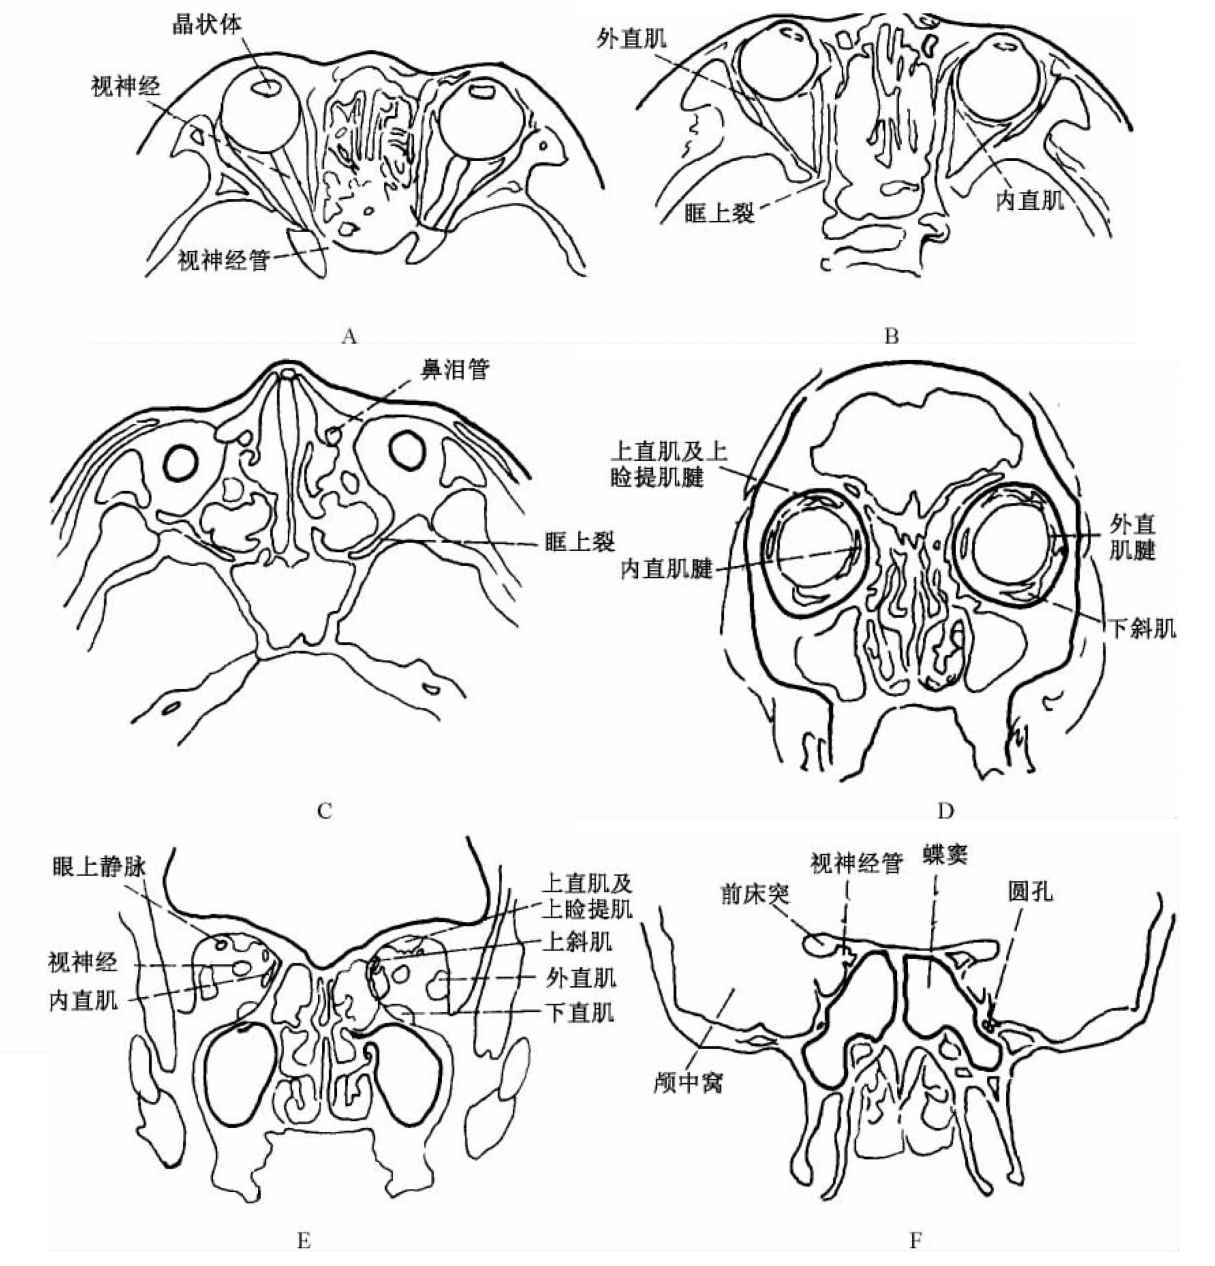
\includegraphics[width=.7\textwidth,height=\textheight,keepaspectratio]{./images/Image00096.jpg}
 \captionsetup{justification=centering}
 \caption{A~F 正常眼眶的横断面和冠状面}
 \label{fig3-1}
  \end{figure} 

\section{先天性病变}

\subsection{眼眶先天性畸形}

单独的眼眶发育畸形并不多见,主要由颅面部发育异常并发的眼眶形态异常。常见疾病如下:

1.颌面骨发育不全:又称为Franceschetti-Klein syndrome和Treacher-Collins
syndrome,主要是下颌骨、颧骨和蝶骨发育不良。

2.颅面骨发育不全:又称为克鲁宗综合征(Crouzon
syndrome),颅腔狭小,下颌骨发育不全,常有独眼畸形、眶顶发育不良和眶腔狭小。

3.尖头并指畸形:又称为Apert syndrome,在眶部表现为眼距宽和眼球突出。

4.骨纤维异常增殖症:较易累及的眶骨为蝶骨大翼、额骨和颧骨等。

5.神经纤维瘤病:可有以下4种表现单独或混合存在。①丛状神经纤维瘤:形成界限不清、形态不规则的软组织肿块,颞肌和眼睑肌肉以及眼外肌不规则增粗变形,强化显著。②眶骨发育不全。③眼眶内肿瘤:主要为视神经胶质瘤,其次是脑膜瘤、神经鞘瘤、神经纤维瘤、神经纤维肉瘤。④眼积水:表现为眼球径增大。

\subsection{眼外肌发育异常}

1.眼外肌缺如:CT可明确显示。

2.眼外肌发育不良:CT表现为患侧眼外肌较对侧细而薄。但是诊断时一定要保证双侧眼眶摆位对称,以免误诊。

\subsection{眼球发育异常}

1.先天性无眼球或小眼球:真正无眼球极少见,其与严重的小眼球只有在组织学上才能区分。小眼球为单侧或双侧,可为单纯眼球较小,其轴长<18mm。一般角膜和视神经均较正常小,但结构正常。有的小眼球伴眼球缺裂或伴眼眶囊肿。

2.先天性囊样眼球:为胚胎发育时视泡未内陷或不完全内陷,形成囊肿样的畸形眼球。CT可显示晶状体异常,囊状眼球的外表仍可附着眼外肌腱。此病难与严重小眼球区别。

3.眼球缺裂:较常见,且多为双侧性。典型的缺裂表现为眼球后壁呈锥形或漏斗状延长,亦可呈葡萄肿样外突,其内为低密度玻璃体。一般眼球和视神经较小,有的完全缺裂,还可以形成囊肿。

4.小眼球伴囊肿:为畸形小眼球内的神经外胚层组织(视网膜内层)通过未闭的缺裂向外突出形成囊肿,属严重的缺裂畸形。眼球可近于正常或很小,囊肿亦可很小或很大。CT可显示小眼球与囊肿间的延续,眶窝常扩大。

\subsection{视神经发育不良}

视神经轴突或视网膜神经节细胞发育不良可为单侧或双侧。

\textbf{【临床表现】}
视力极差、视乳头小,双侧者可有眼球震颤。有的病例伴脑中线结构发育不良、内分泌功能低下、发育延迟、腭裂等,称为中隔-视神经发育不良。

\textbf{【CT表现】}
一般视神经和视神经管均较小,眼窝亦可较小。合并脑中线结构异常者可见透明隔部分或完全缺失,缺损可达第三脑室和侧脑室前角,脑室扩大,胼胝体变薄,视交叉和视束变小。脑白质包括视放射广泛发育不良。以上表现以MR显示为优。

\subsection{永存原发玻璃体增生症}

本病又称原始玻璃体增生症,为胚胎原始玻璃体不能正常退化和胚胎结缔组织过度增生的一种先天性疾病。

\textbf{【病因病理】}
残存的原始玻璃体呈柱状位于晶状体之后与视盘之间称为Cloquet管或玻璃体小管。原始玻璃体内血管可通过晶体后囊的破裂处进入晶体内,使晶体混浊形成白内障。增殖的结缔组织在晶状体后形成纤维斑块,其后面覆以发育不良的视网膜,且可有视网膜剥离。纤维斑块与睫状突相连,将睫状突拉长并拉向瞳孔。混浊肿胀的晶状体可使虹膜晶体隔前移、前房变浅而继发青光眼。玻璃体因纤维增生而混浊,还可有玻璃体出血等继发改变,重型者可继发小眼球。

\textbf{【临床表现】}
散见于足月产婴幼儿,90%为单侧,以白瞳孔或白内障及小眼球引起注意。眼底镜可见晶状体后白色纤维血管膜,扩瞳后可看到延长的睫状体为其特征。

\textbf{【CT表现】}
典型表现为自晶状体后至视网膜间呈带状或三角形异常组织增生,基底在视乳头,尖指向晶体后方,提示玻璃体小管存在。增强扫描病灶显著强化为本病的典型CT表现,有时平扫不易显示需增强扫描予以显示。病侧眼球轻度或中度减小、玻璃体密度增高。肿块密度更高,且无钙化。如有出血或浆液性渗出,眼球内密度可呈分层现象,可有视网膜剥离表现。

病灶无钙化是与视网膜母细胞瘤相鉴别的要点。

\subsection{渗出性视网膜病}

本病又称Coat病,1908年首次由Coat描述。

\textbf{【病因病理】}
为先天性视网膜毛细血管扩张所致。视网膜毛细血管扩张、血管壁增厚、玻璃样变、血管周围有慢性炎性细胞浸润;血管内血清和脂蛋白漏出,导致视网膜增生,出现视网膜下含黄白色结晶的渗出物。因视网膜下大量渗液而继发视网膜剥离,渗出液中见到泡沫细胞可确诊。晚期视网膜及渗出物被机化结缔组织代替。

\textbf{【临床表现】}
好发于20岁以下,80%见于6~8岁,多为单侧发病。视力下降,因视网膜下胆固醇结晶析出而瞳孔发白。眼底镜下可见视网膜血管扩张、迂曲,扭曲呈血管瘤状。

\textbf{【CT表现】}
影像学诊断要点是CT和B超都显示患眼有视网膜脱离征象。因脱离的视网膜下积液蛋白含量高于一般渗出液,故CT多呈半月形高密度区。亦可累及全部玻璃体腔,原因是视网膜完全剥离。无强化,患眼球大小正常,视神经粗细正常,一般均认为患侧眼球内无钙化。但国内也有学者报道可有钙化,因为视网膜血管畸形扩张,有时以微血管瘤出现,有血管瘤就可有钙化;另一方面本病是一种缓慢反复交替的过程,以后形成瘢痕组织成为增殖性视网膜炎,有瘢痕组织就有钙化的可能。

\subsection{牵牛花综合征}

本病是一种较为罕见的非典型和不能分类的视乳头发育异常。由于其眼底镜表现很像一朵盛开的牵牛花而得名,文献上有视乳头先天性发育异常、视神经缺损的命名。

\textbf{【病因病理】}
其病因尚不清楚,可能妊娠2个月前胚裂上端闭合不全或中胚层发育异常所致。病理见视神经缺损伴有特征性视网膜血管异常,且有视神经胶质增生变形和视乳头周围色素沉着,视盘向后进入深的漏斗状的葡萄肿样凹陷,并累及邻近视网膜。可合并一些其他先天性异常如小眼球、永存原发玻璃体增生症、先天性白内障、视网膜剥离等。国外有报道还可合并视网膜、脉络膜缺损,以及晶状体、巩膜缺损。此外,还可伴有中枢神经系统和正中颅面部异常如唇腭裂、脑膨出和胼胝体发育不良等。

\textbf{【临床表现】}
常为单眼发病,罕有双眼者,无性别差异。视力可从正常至完全丧失,多数视力明显减弱。眼底镜表现有特征性:视乳头范围扩大呈粉红色,中央有一大的漏斗状凹陷,被白色绒毛组织充填;视乳头及边缘出现血管异常,细而直,呈放射状;视乳头周围有一灰色隆起的脉络膜-视网膜色素环,环内常有色素沉着。

\textbf{【CT表现】}
视盘呈火山口样凹陷,异常主要局限于视盘是牵牛花综合征最主要的CT特征。视乳头部缺损,局部呈漏斗状或囊状扩张、水样密度,与玻璃体腔相通。缺损周边的巩膜变薄外翻。眼部伴随异常,包括小眼球、先天性白内障、视网膜剥离等。头颅CT扫描还可发现伴随脑部异常。

\textbf{【鉴别诊断】}
①眼球后极部葡萄肿:本病通常指先天或获得性眼球局部膨胀扩张,它不局限在视乳头,也无典型的眼底征象。②伴囊肿的小眼畸形:视网膜脉络膜缺损,巩膜显著扩张,在眼球后部形成一个比眼球还大的囊肿。③视神经肿瘤:牵牛花综合征的视神经增宽呈水样密度,与玻璃体腔相通,可资鉴别。

\subsection{儿童白瞳症的鉴别诊断}

1.视网膜母细胞:最常见,约占47%,也是儿童最常见的恶性肿瘤。1/3两侧发病,多在2岁内出现症状。

CT表现:球内实性肿块,有强化,常发生钙化斑。患侧眼球可增大,球壁及视神经可受侵而增厚、增粗,无眼球缩小的表现。

2.Coat病:是一种良性病变,与视网膜母细胞瘤鉴别要点是发病年龄较大,一般单侧发病,多无钙化,但晚期可有钙化。增强扫描无强化,无眶外侵犯。

3.永存性原始玻璃体增生症:CT表现为残存的玻璃体血管系统以及结缔组织呈条状或三角形密度增高影,自晶状体后面向球后延伸。有强化,可并发视网膜剥离。本病为单侧性,无钙化,常并发眼小畸形,可与视网膜母细胞瘤相鉴别。

4.晶状体后纤维增生症:又称早产儿视网膜病,通常见于早产婴儿吸入高浓度氧气后。

CT表现:玻璃体密度增高,双侧视网膜脱离并不同程度强化。4岁后眼球多萎缩,晶状体、脉络膜和眼球壁可钙化,但眼内少见钙化点。

5.眼犬弓蛔虫病:引起眼内炎症,可表现为白色瞳孔和视网膜脱离。

CT表现:非强化的高密度肿块,占据玻璃腔的大部分。眼外形小,有局限性巩膜增厚并有强化。

6.先天性白内障。

\section{外伤和异物}

\subsection{眼眶爆裂骨折}

眼眶爆裂骨折是指外力作用于眼部,使眶内压力骤然升高导致眶壁内部发生骨折而眶缘无骨折,即骨折的形成与眶内液体压力突然增高有关,不是外力直接作用于眶壁所致。而外力直接作用于眶壁发生的骨折称为眼眶直接骨折,其中发生于内、下壁者必有眼眶前缘的骨折。上述两种骨折同时存在时称为眼眶复合型骨折。

\textbf{【临床表现】}
眼眶爆裂骨折有时可出现复视、眼球运动障碍、视力下降甚至失明,眼球可内陷、突出、固定或斜视等。

\textbf{【CT表现】} 眼眶爆裂骨折的表现如下:

1.直接征象:包括眶壁的连续性中断、粉碎及移位改变,以眶内壁和眶底常见(图\ref{fig3-2})。

\begin{figure}[!htbp]
 \centering
 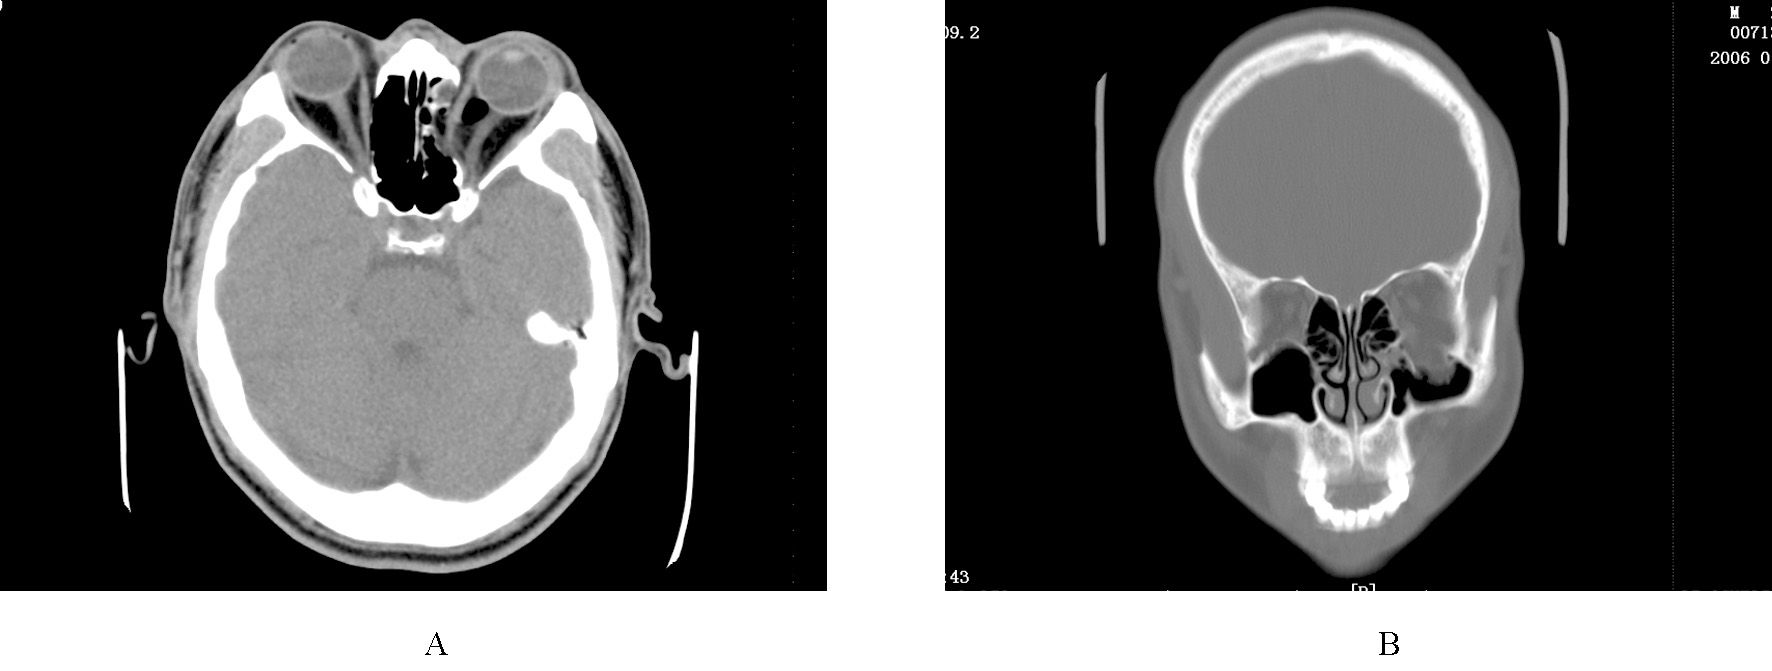
\includegraphics[width=.7\textwidth,height=\textheight,keepaspectratio]{./images/Image00097.jpg}
 \captionsetup{justification=centering}
 \caption{眼眶骨折\\{\small A.左侧眶内壁骨折;B.左侧眶底壁骨折}}
 \label{fig3-2}
  \end{figure} 

2.间接征象:包括眼外肌增粗、移位及嵌顿,眶内容物脱出或血肿形成,并通过骨折处疝入邻近鼻窦内。最常见的间接征象是眶内球后脂肪疝入筛窦。眶内容物疝入上颌窦或筛窦内呈“泪滴征”,有助于眶壁骨质无明显中断或移位的爆裂骨折的诊断。眶内积气更有助于眶壁骨折的诊断。

3.并发症:鼻窦内积血、鼻骨骨折等,也可见鼻窦黏膜肿胀隆起。

\subsection{视神经管骨折}

视神经管骨折临床主要表现为视力明显下降,不少患者表现为失明。

\textbf{【CT表现】} 可分为3类:

1.管内型:即构成视神经管内、外、上、下壁范围内的骨折,可能是减压手术最佳适应证。

2.管外型:指骨折位于管内型骨折以外的视神经骨性通道。包括两个亚型:①颅口型:骨折位于颅内侧视交叉前沟(即蝶窦后壁)至视神经入视神经管处;②眶口型:眶尖处和(或)构成蝶窦外侧壁的蝶骨骨折称为眶口型骨折,此型均合并有眼眶内和(或)外侧壁骨折,骨折处蝶窦内亦可见局限性高密度影。

3.混合型:指管内和管外型骨折合并单处或多处不同部位(不论同侧或对侧)的骨折。

各型骨折均可致视神经受累。CT可见视神经局限性增粗,呈等、低不均匀密度,边缘不规则,还可有高密度出血表现。

\subsection{眼部异物}

\textbf{【分类】}
①金属异物:包括钢、铁、铜、铅及其合金等。②非金属异物:包括玻璃、塑料、橡胶、砂石、骨片和木片等。

\textbf{【临床表现】}
主要为眼部疼痛、不能睁眼,常合并其他眼外伤的症状。如合并眼内炎症则眼部刺激症状和疼痛加剧,视力迅速下降、丧失。

\textbf{【CT表现】}
①金属异物:呈异常高密度影,CT值常>500Hu,并有放射状伪影。②非金属异物:可有高密度和低密度之分。高密度者如砂石、玻璃和骨片等,CT值多>300Hu,一般无明显伪影。低密度非金属异物包括植物类、塑料类。植物类如木质异物的CT值在
-199~-50Hu,其影像与气体类似。塑料类异物CT值为0~20Hu。③CT能较准确显示金属异物,但只能显示较大的低密度非金属异物。④对金属异物大小的测量应以骨窗为准。⑤多平面重建能显示异物的确切位置及与眼环的关系。⑥应注意与球内、球后的异常钙化、人工晶体、义眼及眶内气体相鉴别。

有文献认为,CT可发现小至0.6mm的铁、铜等金属异物;对铝等半透光异物,显影最小径线为1.5mm。对一些合金、玻璃碎屑亦可发现,但对木屑、泥沙等透光性异物不能检出。

\textbf{【并发症】}
包括眼球破裂、视网膜脱离、晶状体断裂或脱位、玻璃体出血、眼球固缩、视神经创伤、眼外肌创伤、眼眶骨折、颈内动脉海绵窦瘘、眶内动静脉瘘以及感染等。

\subsection{眼球损伤}

\subsubsection{眼球机械性损伤的常见CT表现}

机械性眼外伤很常见,如砸伤、拳击伤、撞伤、扎伤、爆炸伤等。

\textbf{【CT表现】}
①眼球体积改变(变大或变小):由球内出血或眼内容物脱出引起;②眼球变形、眼环不连续或部分球壁增厚:可由局部球壁挫伤致水肿、破裂伤或穿孔引起;③玻璃体积血:来自睫状体、脉络膜和视网膜,见玻璃体内斑片状高密度灶;④晶状体密度减低:临床称为外伤性白内障;⑤晶状体位置改变(脱位或脱出);⑥其他:还可见眼球突出、玻璃体混浊、视网膜脱离、前房加深、晶状体形态不整及边缘模糊、眶内积气、球后血肿等改变。以上①~④在眼球挫伤和穿孔伤中均常见。

\subsubsection{眼球破裂伤的CT表现}

眼球受到外力打击致眼内压骤然升高,压力超过眼球壁所能承受的限度时便造成眼球破裂伤,也属机械性损伤。

\textbf{【CT表现】}
①眼环不连续,近80%有此征像,可伴局部不规则增厚(\textgreater{}4mm),且是眼环破裂的依据之一;②前房加深(角膜到晶状体平面的垂直距离)超过4mm或较健侧深超过2mm是后部巩膜破裂的重要征象,可能是由于巩膜破裂后眼压下降,前房内房水吸收所致;③晶状体脱位或缺如;④球内出血、密度增高、球内异物、积气均是眼球破裂的诊断依据;⑤眼球变形缩小,甚至其内部结构无法辨认(图\ref{fig3-3})。

\begin{figure}[!htbp]
 \centering
 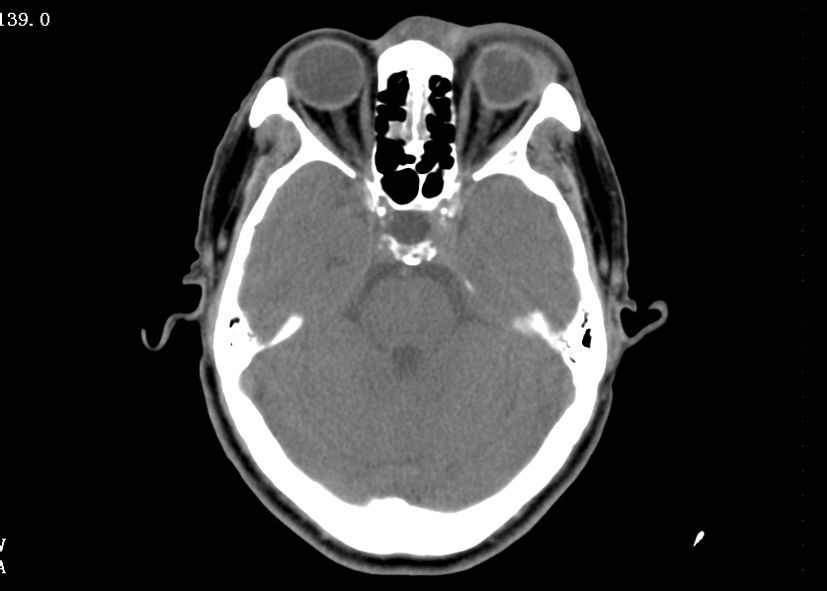
\includegraphics[width=.7\textwidth,height=\textheight,keepaspectratio]{./images/Image00098.jpg}
 \captionsetup{justification=centering}
 \caption{眼球破裂伤\\{\small 左侧眼环不规整,眼球体积略小,球内密度欠均}}
 \label{fig3-3}
  \end{figure} 

\subsection{外伤性白内障}

本病是眼外伤的主要并发症之一,约占36%~52%。

\textbf{【病理】}
穿通伤和钝性伤均可发生。表现为晶状体肿胀、水肿和破裂,是由于晶状体破裂等致房水渗入或震荡、渗透压失常引起晶状体囊下的上皮细胞或晶状体纤维损伤所致。

\textbf{【CT表现】}
晶状体水分增加是晶状体混浊、密度减低的主要原因。密度减低程度与损伤程度和外伤后时间有关。国外有学者测量发现,外伤性白内障患者的晶体CT值平均低于对侧29.5Hu,范围为20.2~46.8Hu,而正常人与对侧平均差为5.97Hu。测量时应在外伤后48h内测定,选择晶状体最大横断面即晶状体中心用4mm\textsuperscript{2}
ROI进行测量,扫描时应采用3mm薄层扫描。

\section{眼眶内炎性病变}

\subsection{眼眶蜂窝组织炎和眼眶脓肿}

本病是眶内软组织或骨膜下的急性化脓性炎症。眶骨膜在眶缘反折附着于上下睑板形成眶隔,可一定程度限制炎症扩展。故可将局限性眶隔前的蜂窝组织炎称为眶周炎症,如在眶隔前后都蔓延则称为眶蜂窝组织炎,可分为肌锥内、外或骨膜下感染。

\textbf{【病因病理】}
大多由鼻窦或眼睑炎症蔓延所致,少数可由外伤、异物、手术后继发感染或泪囊、颌面部炎症引起,偶为血行感染播散所致。致病菌多为溶血性链球菌和金黄色葡萄球菌。眼眶蜂窝组织炎可广泛累及眶内所有组织,甚至海绵窦肿胀增厚,主要为白细胞浸润。眼眶脓肿包括骨膜下脓肿,周围可有较博的壁。发生骨髓炎时可见骨质破坏、骨膜反应或增厚。

\textbf{【临床表现】}
常见眼睑红肿,球结膜充血、水肿,眼球突出和运动障碍,多伴有视力障碍甚至引起视乳头萎缩。如果炎症蔓延至眶尖可引起眶尖综合征;累及海绵窦可形成脓毒性海绵窦栓塞,甚至脑膜炎、脑脓肿;也可发生眶骨骨髓炎。

\textbf{【CT表现】}
①眶隔前眶周炎症表现为眼睑肿胀。泪囊炎可表现为内眦处小囊状肿块。②眶蜂窝组织炎呈眼睑和眼睑后弥漫性软组织肿胀,界限不清,脂肪密度增高。眼外肌肿胀、肥厚,泪腺增大,部分有眼球壁增厚。病变与眼外肌相比呈等密度或略低密度。③增强后呈不均匀显著强化。④眶内脓肿(包括骨膜下脓肿)表现为圆形、椭圆形或梭形低密度(与眼外肌相比),密度不均,增强后脓肿壁强化。⑤骨髓炎表现为眶骨低密度骨质破坏、骨膜反应和骨质增厚。

\textbf{【鉴别诊断】}
骨髓炎骨质破坏与增生同时存在并结合临床不难与转移瘤相鉴别。眶内囊虫病呈高密度头节与低密度囊泡应注意与脓肿鉴别。

\subsection{眼球筋膜炎}

\textbf{【病理分类】}
①浆液性:病因不明,一般认为属自身免疫性疾病,多发生于双眼;②化脓性:多因邻近结构化脓性炎症蔓延或外伤感染所致。

\textbf{【临床表现】}
发病急、进展快,疼痛、结膜充血水肿。如果邻近的眼外肌受累则可有眼球运动受限,视力多不受影响。

\textbf{【CT表现】}
局部球壁增厚,部分可伴眼外肌增粗;增强后病灶明显强化。化脓性如治疗不及时可形成急性眶蜂窝组织炎。

\subsection{眼眶特发性炎症}

本病又称眼眶炎性假瘤、眼眶非特异性炎性假瘤,是一种原因不明的非特异性炎性病变,目前认为是一种免疫反应性疾病。它不包括Wegerner肉芽肿、硬化型血管瘤、外伤、鼻窦炎等引起的眼眶炎性病变。

\textbf{【病理】}
早期为水肿和轻度炎性浸润。浸润细胞包括淋巴细胞、浆细胞和嗜酸性细胞,随炎症进展逐渐纤维化。可合并其他部位的纤维化病变,如纤维性纵隔炎、腹膜后纤维化、慢性纤维性甲状腺炎、硬化性胆管炎等。

\textbf{【临床表现】}
多发病于10~40岁。典型表现为发病较快,常反复发作,有眼球突出,眼睑肿胀及球结膜水肿、疼痛,眼球活动受限及复视、视力减退等,可出现眶尖和海绵窦综合征。多为单侧发病,可为双侧。临床可分为急性和慢性2种。急性者类固醇治疗效果较好,尤其肌炎型和泪腺炎型;慢性者放疗有时效果较好。本病不宜手术和取活检。

\textbf{【CT分型】} 其CT分型方法较多:

1.国外有学者将其分为5型:①前部假瘤;②后部假瘤;③弥漫型;④泪腺炎型;⑤肌炎型。

2.国外亦有人将其分为2型:①局限型;②弥漫型。弥漫型又分为急性和慢性2种临床亚型。

3.国内有学者将其分为5型:①肿块型;②泪腺炎型;③肌炎型;④弥漫型。其中肿块型又分为前部型和后部型。

\textbf{【CT表现】}
主要表现为眶内局限性或弥漫性软组织影,边缘清晰或不清,有不同程度强化。病变可累及眶内单个或多个结构,眼环及球后脂肪间隙常受累。多为单侧发病,有人报道双侧者多为泪腺炎型。

1.眼睑肿胀和眼球突出:为最常见的表现。约半数有眼球侵犯,常表现为球壁增厚,为巩膜及眼球筋膜炎所致。增厚范围与炎症接触眼球的范围相一致,且增厚处显著强化是与Graves眼病鉴别的一个较特异征象。

2.泪腺增大:多与眶内其他部位侵犯并存。急性者显著强化,慢性者应注意与淋巴瘤、泪腺肿瘤、结节病、干燥综合征等相鉴别,但有时较难鉴别。

3.眼外肌侵犯:很常见。有的仅单一眼肌受侵,以上直肌和内直肌较为多见。常为多肌侵犯伴视神经、眶脂肪或泪腺病变。眼外肌增厚为弥漫性,可累及肌肉全部,亦可为一部分。眼外肌眼球附着处增厚是本病较典型的征象。

4.视神经增粗:少见。边缘不规则,为视神经鞘炎所致,多与其他病变并存。

5.眶内脂肪炎症浸润:较常见。内有网状密度增高影,为纤维间隔增厚所致;出现不规则小结节状密度增高影,为肉芽组织增生所致。

6.其他:偶见眶窝增大、眶骨硬化增厚或骨质吸收破坏。应注意与恶性肿瘤和肉芽肿病变相鉴别。

\textbf{【鉴别诊断】}

1.淋巴瘤:在眼眶内泪腺是其好发部位。可以是原发或继发,对放疗、化疗敏感。①在眼肌圆锥后也可呈浸润性生长,使正常软组织之间的界限消失,有强化。与眶内炎性假瘤很相似,两者组织学、临床及CT表现均很难鉴别。②在泪腺表现为泪腺窝区密度增高的肿块,亦有强化。与眶内炎性假瘤鉴别有时困难。

2.Graves眼病:与眶内炎性假瘤的鉴别见表\ref{tab3-1}。

\begin{table}[htbp]
\centering
\caption{眼眶炎性假瘤与Graves眼病的鉴别诊断}
\label{tab3-1}
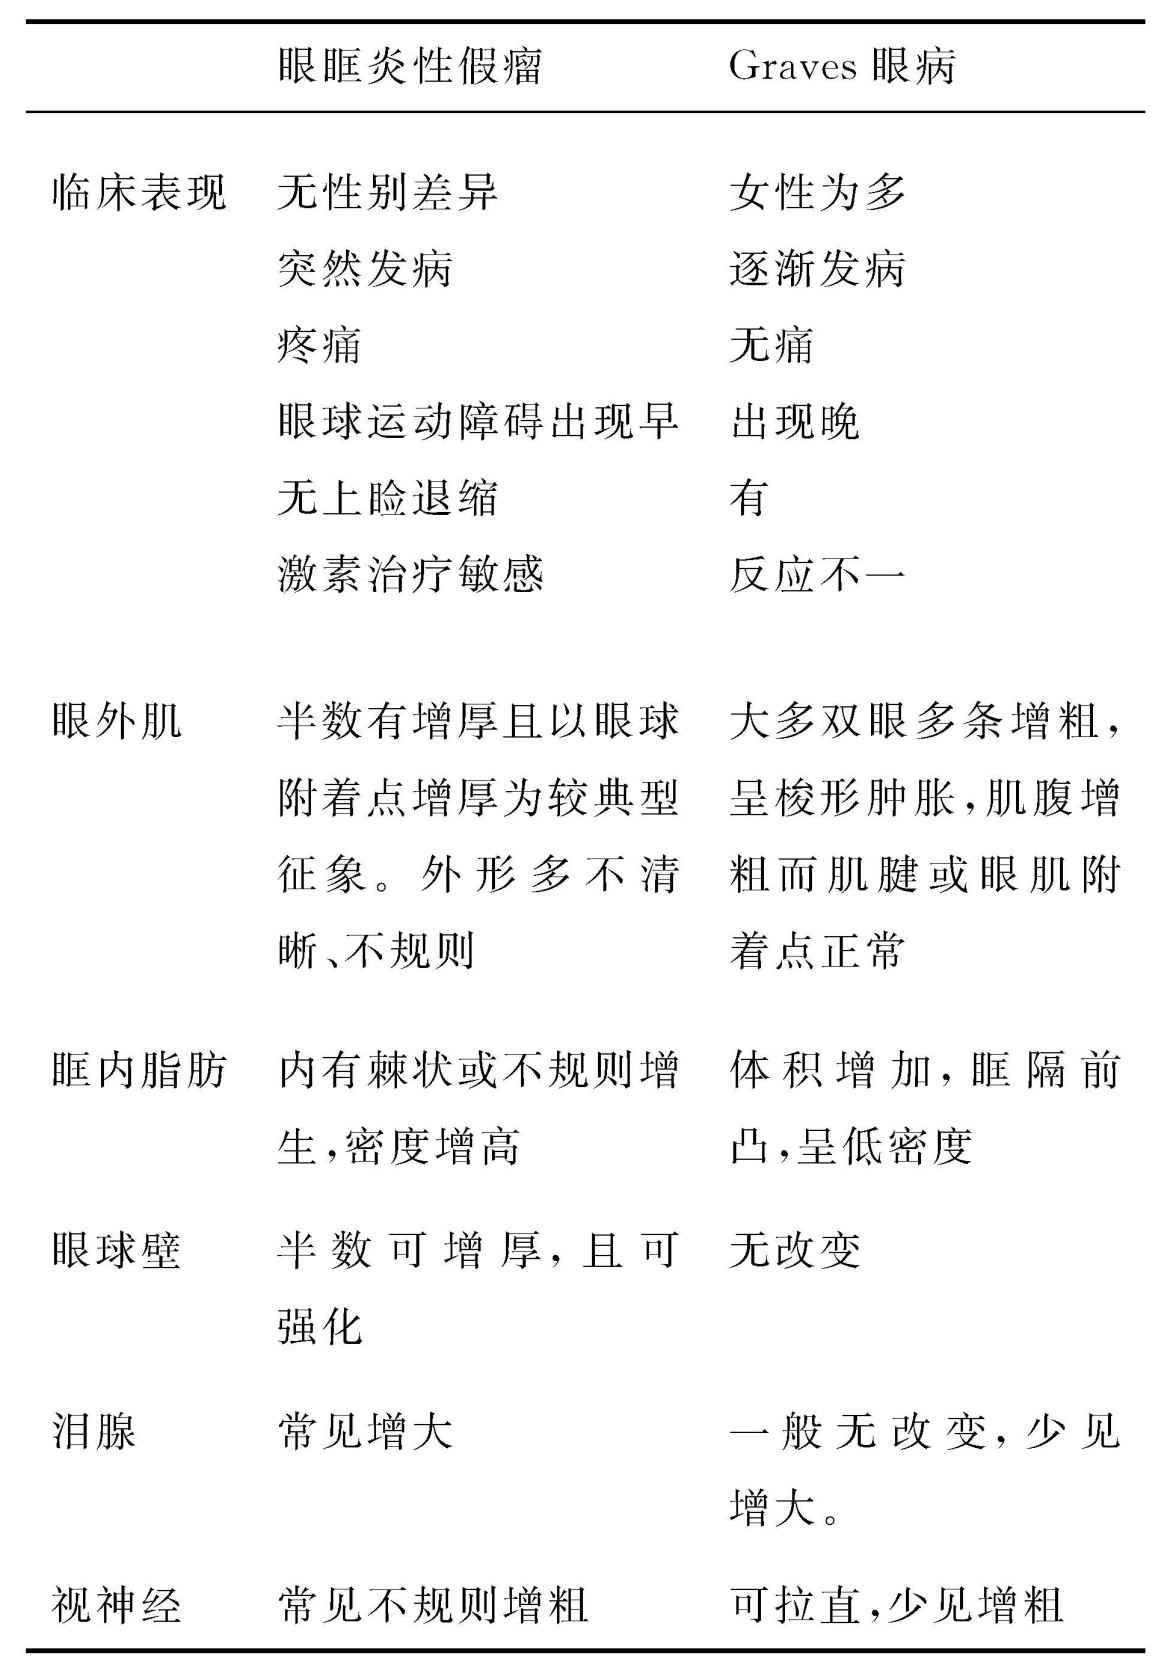
\includegraphics[width=\textwidth,height=\textheight,keepaspectratio]{./images/Image00099.jpg}
\end{table}

\subsection{Graves眼病}

Graves眼病又称甲状腺眶病、内分泌性突眼、甲状腺性突眼,这是除蜂窝组织炎和外伤外单侧或双侧突眼的常见原因。可发生于甲状腺功能亢进期或其前后,亦可见于甲状腺功能减低者,故很多患者并无甲亢。有学者将甲状腺功能异常伴有眼征者称为Graves眶病;甲状腺功能正常者称为眼型Graves病。发病机制尚不明确,有甲状腺素---促甲状腺素分泌紊乱和抗体自身免疫学说。

\textbf{【病理】}
主要改变为眼外肌肥厚和眶内脂肪体积增加。大多有淋巴细胞和浆细胞浸润,有散在的肥大细胞,以及黏多糖沉积。最后眼外肌纤维化。

\textbf{【临床表现】}
本病发作慢,可出现上睑退缩(凝视)、迟落,部分产生复视、眼球突出等症状。重型可致角膜暴露甚至发生溃疡,视神经受压甚至萎缩以至视力减退。多为双侧发病,单侧者占5%~10%。

\textbf{【CT表现】}
①典型表现为双侧多发眼外肌肥大和眶内脂肪体积增加,致眶隔前移及眼球突出。②眼外肌以下直肌最常受累,其次为内直肌、上直肌和提上睑肌,偶尔累及外直肌。以肌腹增粗而其肌腱及眼附着部不增粗为特点(图\ref{fig3-4}),少数也侵及肌腱。增强扫描早、中期增粗的眼外肌轻至中度强化,到晚期纤维化时则无强化。③少数可有眶内脂肪密度增高、泪腺增大和眼睑水肿。

\begin{figure}[!htbp]
 \centering
 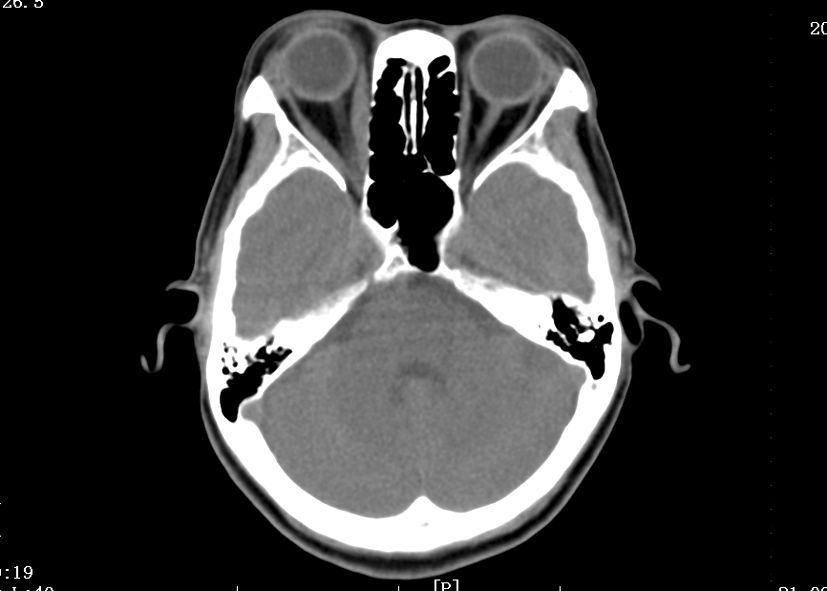
\includegraphics[width=.7\textwidth,height=\textheight,keepaspectratio]{./images/Image00100.jpg}
 \captionsetup{justification=centering}
 \caption{Graves眼病\\{\small 右内直肌、外直肌均增厚,以内直肌为著;左侧内直肌略增厚;均为肌腹增粗}}
 \label{fig3-4}
  \end{figure} 

应注意与肌炎型炎性假瘤、动静脉瘘、转移瘤、淋巴瘤等相鉴别。

\subsection{泪腺炎}

本病有急慢性之分,以慢性多见,多为双侧发病。

\textbf{【病因】}
急性者多继发于某些急性传染病,慢性者常为结核菌和沙眼病毒引起。

\textbf{【临床表现】}
泪腺肿大使上睑外上部分隆起,眼球向外上转动受限,可出现复视。

\textbf{【CT表现】}
一侧或两侧泪腺呈杏仁状或椭圆形增大,眼球可向内、下或前移位。急性者肿大的泪腺多较对侧密度略低,且欠均匀,界限不清,邻近软组织常肿胀。慢性者多呈等密度,界限清楚。结核感染所致者可见斑点状钙化,且常伴耳前淋巴结肿大。增强扫描可有不同程度强化。

\textbf{【鉴别诊断】}
应注意与其他一侧或两侧泪腺肿大的疾病如淋巴瘤、混合瘤、结节病、米枯力兹病相鉴别。

\subsection{视神经炎}

本病有急、慢性两类,以慢性较多见。

\textbf{【病因】}
急性者多由邻近炎症如眼眶蜂窝组织炎、鼻窦炎、颅底脑膜炎等所致,也可见于铅、砷、甲醇中毒。慢性者多由维生素缺乏、糖尿病、脱髓鞘病变引起。眶内炎性假瘤及内分泌性突眼亦可影响视神经。

\textbf{【临床表现】} 显著的视力下降,突发性中心视野缺损伴眼眶疼痛。

\textbf{【CT表现】}
视神经正常或弥漫性增粗(但不像肿瘤那样显著),与炎症程度有关。平扫密度与健侧相似,增强后可见轻度强化,部分可见“双轨”征。

\section{眼及眼眶部肿瘤}

\subsection{概述}

眼及眼眶部在组织学上含有外、中、内胚层演变来的各种组织,因而肿瘤种类很多,名称亦较复杂。按其解剖部位可大致分类(见表\ref{tab3-2})。

\begin{table}[htbp]
\centering
\caption{眼及眼眶部的常见肿瘤}
\label{tab3-2}
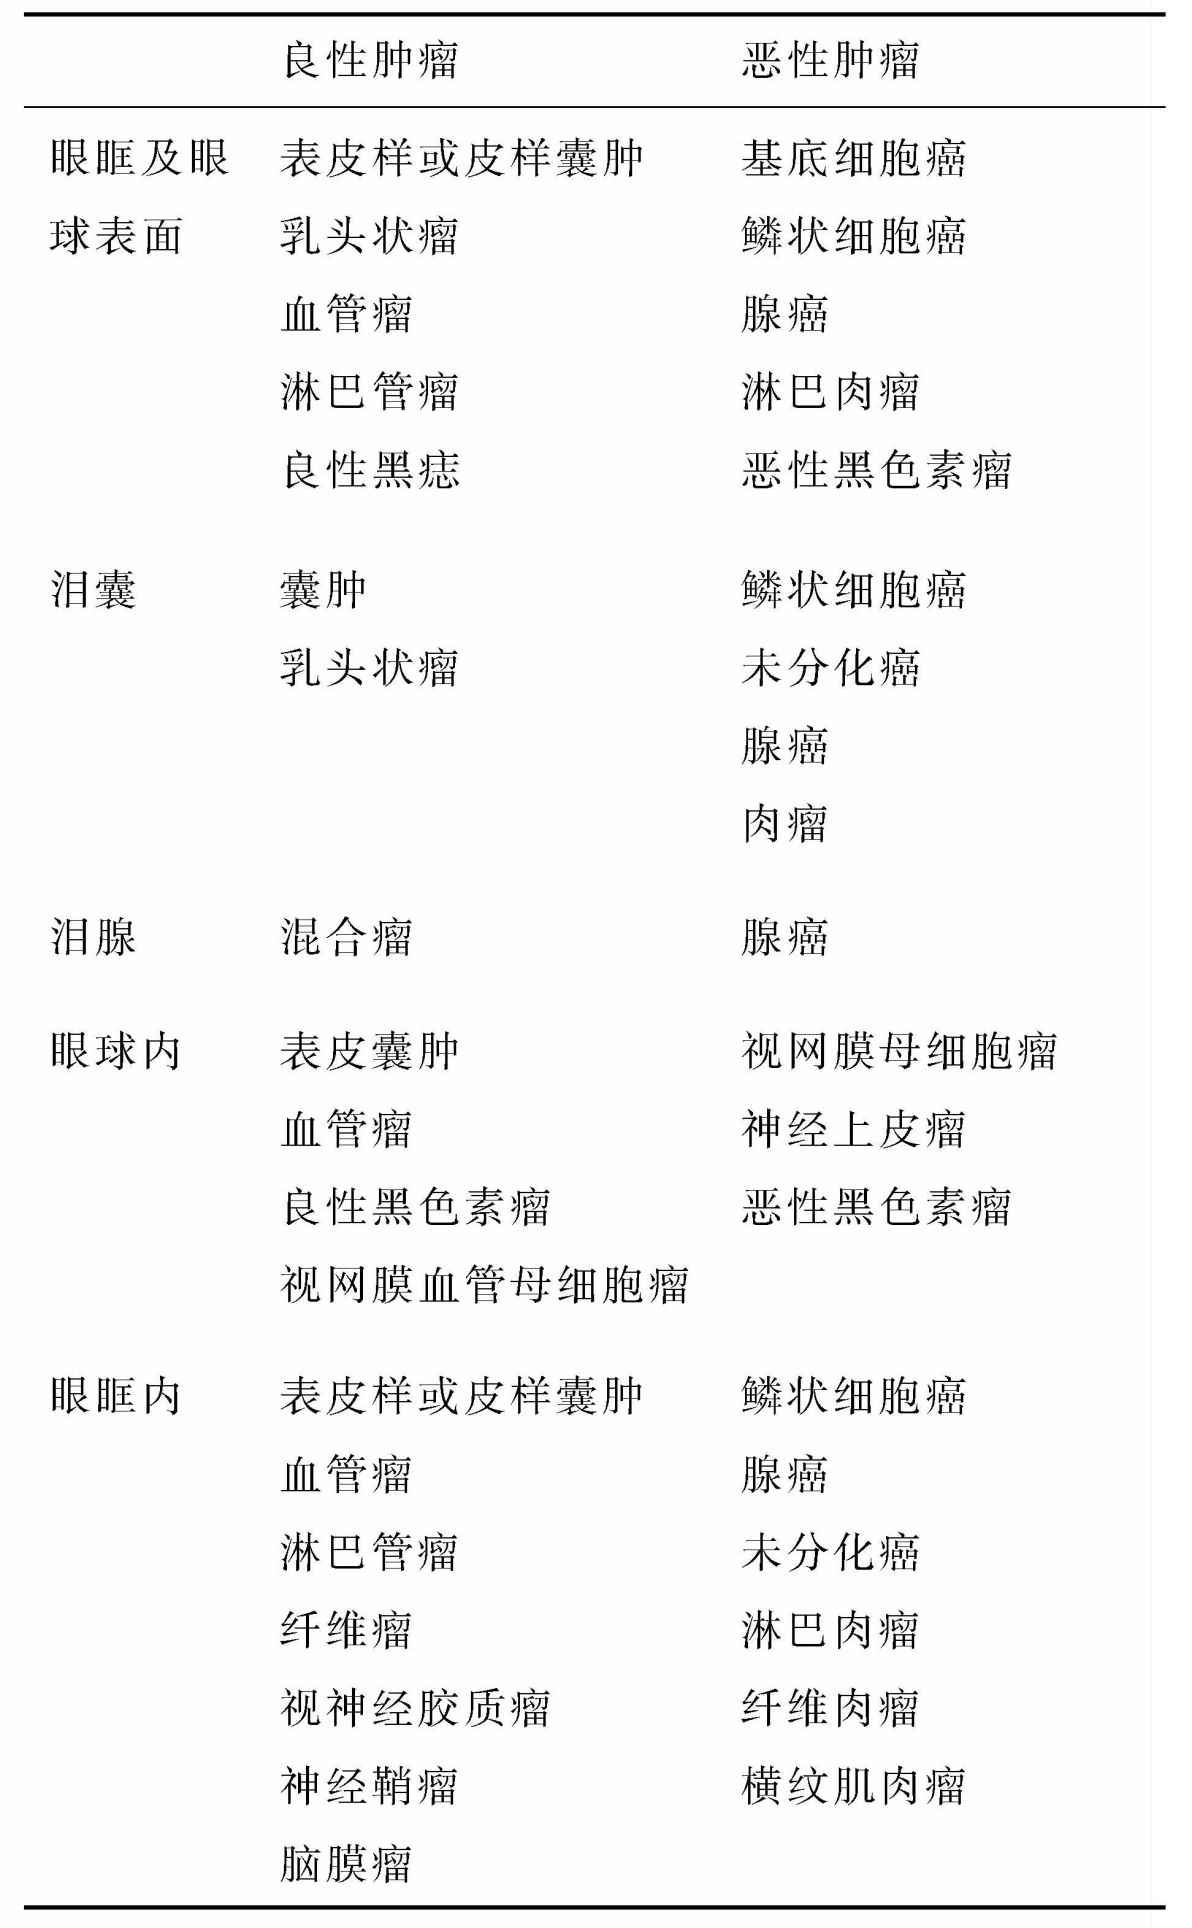
\includegraphics[width=\textwidth,height=\textheight,keepaspectratio]{./images/Image00101.jpg}
\end{table}

1.眼球内肿瘤:一般指视网膜和葡萄膜的肿瘤,晶状体、玻璃体无原发肿瘤。如视网膜母细胞瘤多见于小儿,CT平扫显示眼环后部高密度肿块,突向眼球内外,肿块常发生斑点、斑片状钙化,累及视神经时表现视神经增粗。而葡萄膜恶性黑色素瘤多见于成人,无钙化。

2.眼眶内肿瘤:①良性肿瘤:CT表现为高密度或低密度肿块,边缘清楚、轮廓光整、密度均匀,邻近眶壁者可造成局部骨质光滑凹陷,边缘硬化,而无虫噬样骨质破坏。特征性表现为血管瘤在肿块中见到静脉石;脑膜瘤肿块中见到不定形钙化,邻近眶壁有骨增生或破坏;泪腺混合瘤肿块位于泪腺窝;皮样囊肿CT值<10Hu。②恶性肿瘤:CT表现为肿块形态不规则、密度不均匀、边缘不清楚,常引起眶壁骨质破坏,并向颅内、鼻窦或颞窝延伸。

3.眶壁、鼻窦及颅内肿瘤向眶内延伸:有以下特点:①肿块最大径或大部分在眶周结构内;②具有眶周结构肿瘤的特点;③肿块部分侵入眶内。

此外,许多肿瘤可发生于或侵及眶骨,如眶内脑膜瘤、绿色瘤、神经纤维瘤病、皮样囊肿和转移瘤,还有血管瘤、骨瘤、骨软骨瘤、软骨瘤、骨巨细胞瘤、骨髓瘤、骨纤维异常增殖症、骨化性纤维瘤、组织细胞增生症等;鼻窦的囊肿及鼻腔、鼻窦、鼻咽部肿瘤亦可侵及眼眶;颅内的脑膜瘤、垂体瘤、视交叉胶质瘤等也可侵及眼眶。

儿童眶部肿物(不包括眼球)以良性为多,占88%~92%,恶性占8%~12%。儿童眶内肿物以囊性肿瘤(主要是皮样囊肿、表皮样囊肿、畸胎瘤及淋巴管瘤)、炎性肿块、脉管性肿瘤(毛细血管瘤和淋巴管瘤)、视神经胶质瘤常见,其中以皮样囊肿和表皮样囊肿最常见。与成人相比,海绵状血管瘤、视神经鞘脑膜瘤、泪腺肿瘤在儿童均少见;恶性肿瘤以横纹肌肉瘤多见,少见的有成神经细胞瘤、视网膜母细胞瘤转移瘤、绿色瘤、淋巴瘤(见表\ref{tab3-3})。

\begin{table}[htbp]
\centering
\caption{儿童眶部肿物(不包括眼球)}
\label{tab3-3}
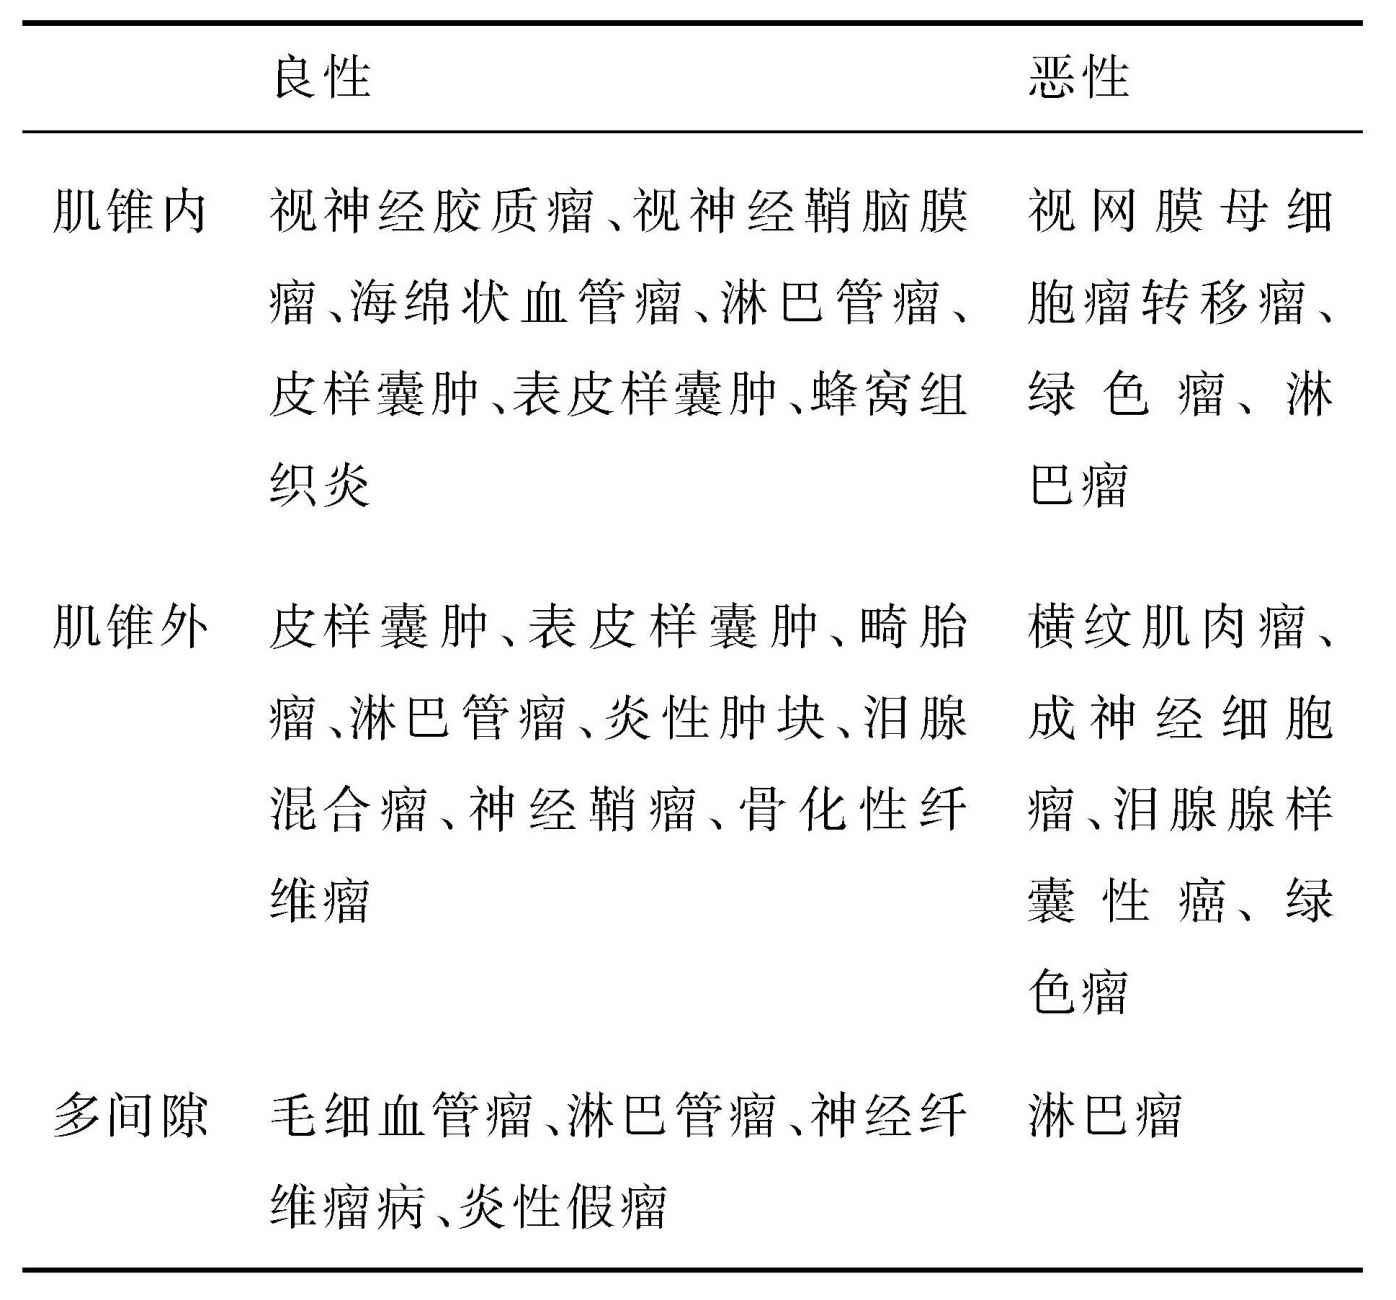
\includegraphics[width=\textwidth,height=\textheight,keepaspectratio]{./images/Image00102.jpg}
\end{table}

\subsection{视网膜母细胞瘤}

本病系来自视网膜细胞的胚胎性恶性肿瘤,又称为成视网膜细胞瘤,具有先天性和遗传性,是婴儿中最常见的眼内恶性肿瘤。患者约98%为儿童,以5岁以下特别3岁以下多见,有的生后即被发现,10岁以上很少见。

\textbf{【病理】}
按生长部位分为:①内生型:起源于视网膜内核层并向玻璃体内生长;②外生型:起源于视网膜外核层,沿视网膜下间隙及脉络膜方向生长,引起视网膜剥离。显微镜下分为:①未分化型:恶性程度较高,瘤细胞形态差异很大,呈圆形、椭圆形、多角形或不规则形,瘤细胞围绕在血管的外围可形成珊瑚样或指套样排列,称为假菊花形排列;②分化型:恶性程度较低,瘤细胞呈方形或低柱状,围绕一个中央腔隙形成一个菊花形排列,分化更好的可见类似光感受器的成分。

\textbf{【临床表现】}
多见于5岁以下幼儿,绝大多数为3岁内起病。以单眼为多,约18%~40%可双眼先后或同时发病,约10%可出现不治自愈的现象。临床表现为视力减退或丧失、经瞳孔可见黄白色反光(俗称“猫眼”)、斜视、眼球红痛、突出,晚期可见眼球破溃。不少患者死于颅内侵犯及淋巴或血行转移(颅面骨、躯干骨、肝和肺等全身各处)。临床可分为眼内生长期、青光眼期、眼外期及转移期。

\textbf{【CT表现】}
平扫可见眼环后部高密度肿块,其内有斑点、斑片状钙化有定性意义,有时整个肿瘤完全钙化,肿瘤钙化率达90%以上(图\ref{fig3-5})。增强扫描未钙化部分有强化。较大肿瘤可致眼球膨大,并可穿破角膜和巩膜进入眶内,甚至几乎充满眼眶。肿瘤沿视神经向球后蔓延,可见视神经不规则增粗、球后肿块,甚至侵及颅内。

\begin{figure}[!htbp]
 \centering
 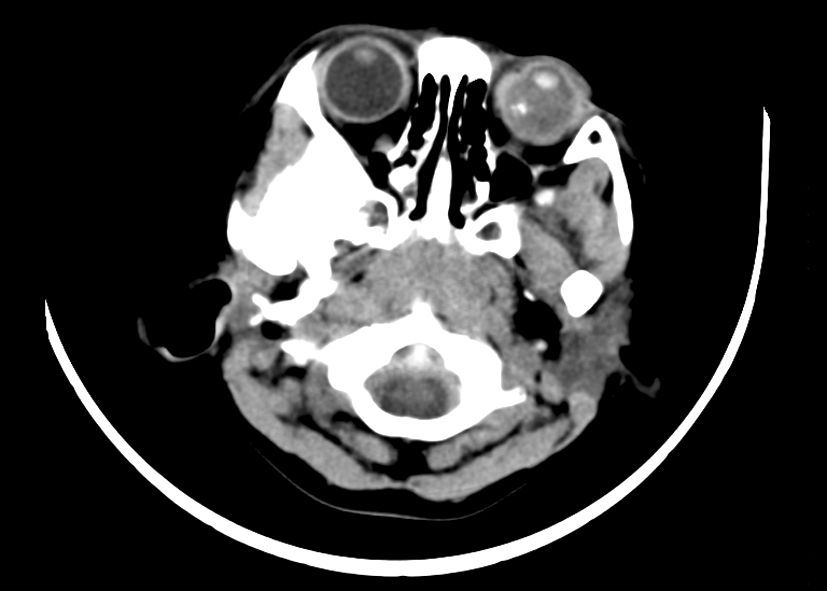
\includegraphics[width=.7\textwidth,height=\textheight,keepaspectratio]{./images/Image00103.jpg}
 \captionsetup{justification=centering}
 \caption{视网膜母细胞瘤\\{\small 左侧球内有高密度肿块,其内有斑片状钙化}}
 \label{fig3-5}
  \end{figure} 

某些视网膜母细胞瘤患者,可伴发组织学与视网膜母细胞瘤类似的颅内松果体瘤及鞍上或鞍旁的原发性视神经母细胞瘤,称之为“异位性视网膜母细胞瘤”;可出现于双眼视网膜母细胞瘤患者,故又称为“三侧性视网膜母细胞瘤”。三侧性视网膜母细胞瘤并非视网膜母细胞瘤颅内转移,也不是视网膜母细胞瘤与颅内松果体瘤及鞍上或鞍旁的原发性视神经母细胞瘤的偶然共生,而被认为是视网膜母细胞瘤基因异常表达的另一种形式。

\textbf{【鉴别诊断】}

1.眼球痨:是眼睛失明以后的晚期钙化和眼球萎缩,可见于婴幼儿。病因有外伤、慢性眼内炎症(如结核)、手术后遗、视网膜反复出血及放疗后。CT表现为眼球不规则变小并广泛钙化。眼球萎缩与视网膜母细胞瘤有别。

2.晶体后纤维增生症:发生于早产生儿吸氧史者,一般为双眼。在晶体后与视网膜间有条索状的机化纤维增生带,玻璃体密度高,视网膜常剥离。4岁后眼球多萎缩,晶状体、脉络膜和球壁可钙化,但眼内少见钙化点。

3.Coat病:多见于6~8岁儿童,为视网膜先天异常(毛细血管扩张)伴视网膜下渗出,一般单侧发病。视网膜呈翼状或V形剥离。一般无钙化,但晚期可钙化。增强扫描无强化,亦无眶外侵犯可资鉴别。

4.原始玻璃体增生症:虽表现为晶体后条状、三角形有强化的密度增高影,但可根据无钙化、伴眼小畸形而予以鉴别。

5.视网膜剥离:与肿瘤密度相似,呈新月状,典型者呈“V”形、翼状。增强后视网膜下积液不强化,仅见脱离的视网膜强化,据此多可鉴别。

6.视乳头玻璃小体:也称视神经小疣,是成人眼球局限性钙化最常见的原因,一般为双侧对称。CT表现视乳头表面的孤立圆形高密度钙化。

此外,应注意与眶内寄生虫病、脉络膜骨瘤和转移瘤(后两者多见于成人)相鉴别。脉络膜血管瘤甚至恶性黑色素瘤亦可有钙化,前者可见于儿童,但后者见于成人,也应注意鉴别。

\subsection{葡萄膜恶性黑色素瘤}

本病是发生在黑色素细胞的恶性肿瘤,是成人眼球内最常见的原发性恶性肿瘤,儿童少见。85%发生于脉络膜,9%发生于睫状体,6%发生于虹膜。

\textbf{【病理】}
可分为有黑色素的和无黑色素的。其生长表现为结节型和弥漫型。①结节型:早期局限,生长到一定高度,其顶端突破玻璃膜,由于受玻璃膜裂口的限制,头部在视网膜下迅速生长,形成头大、颈狭和基底广的蘑菇状肿块,并可继发视网膜剥离,其血管丰富。②弥漫型:少见,约占5%,沿脉络膜平面生长可达1/4以上甚至整个脉络膜。有学者将脉络膜黑色素瘤按大小分为小肿瘤(高度≤10mm)、中等大小肿瘤(高度11~15mm,常为典型的蘑菇形)、较大肿瘤(高度\textgreater{}15mm,可占据整个眼球)。发生于睫状体和虹膜者较小。显微镜下肿瘤主要由梭形细胞A型、梭形细胞B型和上皮样细胞组成。

转移途径:本病易侵及血管,约半数发生血行转移,大多转移至肝和腹腔脏器,次为肺和骨,也可转移至皮下淋巴结。

\textbf{【临床表现】}
好发于中年人,平均年龄50岁,男女发病率相近,多为单眼发病。临床表现与肿瘤位置和体积有密切关系。靠近周边部脉络膜或较小的肿瘤早期症状不显著。位于眼球后部或黄斑部者,早期就可出现视力下降、视野缺损、玻璃体漂浮物等症状。伴广泛视网膜脱离则视力明显下降甚至失明。眼底镜局限型呈棕黑色球形隆起;弥漫型类似转移瘤,甚至易误诊为葡萄膜炎、青光眼或视网膜剥离。

\textbf{【CT表现】}
虹膜、睫状体黑色素瘤一般较小,CT很难显示。发生于脉络膜者,早期多见球后极部扁豆状或半球状不典型肿块;随肿瘤生长突破玻璃体形成典型的“蘑菇”状肿块。肿块密度与眼环相近,偶有钙化(关于其钙化报道不一致)。增强后肿瘤多为中度以上均匀强化,如肿块有坏死囊变则强化不均。继发的视网膜剥离呈半月形,CT难以区分,增强扫描视网膜强化不显著有助于鉴别。MR其短T\textsubscript{1}
短T\textsubscript{2} 信号具有特征性。

\textbf{【鉴别诊断】}
需与脉络膜血管瘤、转移瘤、视网膜下积液、黑色素细胞瘤(罕见的良性肿瘤,是一种特殊类型的色素痣,又称大细胞样痣)等鉴别,主要依靠其典型的MR特征并结合临床(包括眼底镜)、B超和荧光造影等鉴别。此外,睫状体神经鞘瘤是睫状体神经细胞异常增生所形成的良性肿瘤,非常少见;CT表现眼球前份睫状体区软组织肿块,形态不规则,与晶状体分界不清;临床及CT对其良恶性及与其他肿瘤鉴别困难,靠针吸或活检组织学确诊。

\subsection{脉络膜骨瘤}

本病是由成熟骨组织构成的良性肿瘤。

\textbf{【病因病理】}
病因不明,可能为代谢、遗传、感染或外伤所致脉络膜间质组织或化生的色素上皮异位骨化。表现为脉络膜毛细血管附近的组织或全层组织内有海绵状松质骨骨瘤,由相互连接的骨小梁及单层内皮细胞形成的大血窦组成。

\textbf{【临床表现】}
好发于20~30岁女性,多为单眼发病。可无任何症状或轻微视力减退、视物变形和视野缺损。大多数病灶位于视乳头旁,亦可累及黄斑部。眼底镜呈橘黄色或灰色局部隆起,表面有血管分支,甚至有视网膜剥离。

\textbf{【CT表现】}
眼球后极部点状、短线状或纺锤形骨化影,边缘清晰光整,少数可伴视网膜剥离。

\textbf{【鉴别诊断】}
①视乳头玻璃体疣:多为双侧,病变在视乳头表面。②脉络膜血管瘤:未钙化部分强化显著。还应注意随访,与钙化的脉络膜黑色素瘤相鉴别。

\subsection{脉络膜血管瘤}

本病是在血管发育不良的基础上形成的良性肿瘤。

\textbf{【病理】}
本病属于良性、血管错构瘤性病变。病理上可分为局限型或孤立性血管瘤(病理称海绵状血管瘤)和弥漫型(性)血管瘤(病理又称毛细血管型血管瘤)两类,后者少见,通常伴有Sturge-Weber综合征。局限型多位于眼球后极部,呈梭形或椭圆形。

\textbf{【临床表现】}
局限型多发生在20~50岁,早期一般无症状;眼底见橘红色的肿块,可有视网膜脱离。弥漫型多见于10岁以下儿童;眼底呈橘红色,界限不清,易并发广泛视网膜剥离,通常伴有脑颜面血管瘤病。

\textbf{【CT表现】}
平扫难以显示,表现为局限性或弥漫性脉络膜增厚。最具特征的是增强后明显强化。肿瘤的高度一般较小,应首选B超或MR检查。

\subsection{眼球内血管性病变}

1.脉络膜血管瘤(见上述)

2.视网膜血管母细胞瘤:可单独发生,也可以是Von Hippel
Lindau综合征的一部分。为一种发生于视网膜、视神经的良性毛细血管瘤。Von
Hippel
Lindau综合征有遗传倾向,半数双侧发生。眼底镜可见球形肿块以及扩张的供血动、静脉。肿瘤增大可致浆液渗出、玻璃体出血、视网膜剥离。

CT表现:病变多发,常因太小而不易发现。眼球壁局部增厚和密度增高。Von
Hippel
Lindau综合征的眼外表现有:小脑、中脑或(和)脊髓血管母细胞瘤,肾和胰腺肿瘤,多发内分泌瘤。

3.Wybun-Mason综合征:又称先天性视网膜动静脉血管瘤,有家族性。眼底可有渗出和出血,眼动脉常增粗。

CT表现:单侧眼球内不规则扭曲状肿块,可增强,可伴眼眶、颜面及颅内中脑等处类似的血管畸形。

4.Sturge-Weber综合征:可伴同侧脉络膜弥漫性血管瘤和颅内血管瘤。

\subsection{脉络膜转移瘤}

脉络膜血运丰富,故眼球内转移瘤多发生于脉络膜。

\textbf{【病因病理】}
全身癌肿均可经血行转移至此。原发癌以乳癌和肺癌最常见,泌尿生殖系、胃肠道和皮肤部位的癌肿亦可转移至眼内。表现为脉络膜弥漫扁平状增厚,偶为圆顶状增厚。

\textbf{【临床表现】}
本病发病率约为1/10万。可单眼或双眼发病,常诉眼痛、头痛,视力可下降。眼底可见灰黄色或黄白色不规则单个或多个结节,可继发视网膜剥离。

\textbf{【CT表现】}
CT显示率不高,应首先行B超和MR检查。眼环较广泛扁平增厚,少数呈结节状隆起。常伴视网膜下积液和V形、弧形或半球形的高密度视网膜剥离影。但积液内如有蛋白及血液渗出时CT值高于水,平扫不易区分肿瘤与渗液,且积液量大而肿瘤小时易单纯诊为视网膜剥离;增强扫描时转移灶强化,而积液无强化。有的病例可见视神经增粗及球后脂肪内肿块。

上述表现均无特异性,与脉络膜黑色素瘤及血管瘤等鉴别困难。如患者有原发癌病史且双眼多发有助于诊断。

\subsection{视神经胶质瘤}

原发于视神经的肿瘤有视神经胶质瘤和视神经脑膜瘤,以前者多见,两者之比为3∶1~4∶1。视神经胶质瘤占视神经原发肿瘤的80%,占所有眼眶肿瘤的4%,占所有颅内肿瘤的2%,占所有颅内胶质瘤的4%。本病伴发神经纤维瘤病者达15%~50%。

\textbf{【病理】}
视神经胶质瘤起源于视神经内神经胶质,属于良性或低度恶性肿瘤,发生于成人者恶性程度较高。大多为分化较好的星形胶质细胞瘤,少数为少支胶质细胞瘤。有学者根据发病部位分为球内型、眶内型和颅内型。肿瘤可发生于视神经通路的任何部位,以视神经、视交叉和视束(合称为前视路)为好发,故可通过视神经管扩展,但尤以眶内段好发。原发于颅内者可侵犯下丘脑和视束,扩展至外侧膝状体和枕叶。约1/3的病侧同时有视神经纤维瘤病,一般不引起血行和淋巴转移。

\textbf{【临床表现】}
视神经胶质瘤75%发生于10岁以内儿童。患眼视力减退为最早症状,并可出现视野缺损,随病灶增大而眼球突出。如累及颅内可有下丘脑异常症状及阻塞性脑积水。眼底镜常见较明显的视神经萎缩、视乳头水肿。

\textbf{【CT表现】}
患侧视神经呈局限性梭形或管形(弥漫一致性)增粗,亦可呈结节状、哑铃状或椭圆形增粗,增粗的视神经迂曲,肿瘤边界清楚。肿瘤平扫与脑实质呈等密度,增强扫描呈均匀或不均匀性轻、中度强化,少数不强化。有些肿瘤内有黏液样变或囊性变而呈低密度,增强扫描强化不均匀。一般无钙化,但少数有小的钙化。大的肿瘤可累积整个眼眶,并可侵及眼球和脑组织。晚期可有视神经管或眶锥等部位的扩大和骨质吸收破坏。该瘤常侵及颅内段及视交叉,在鞍上池形成肿块。

\textbf{【鉴别诊断】}
①视神经鞘脑膜瘤:本病强化明显,而视神经不强化,可见“双轨”征,并可引起眶骨骨质增生是与胶质瘤的鉴别要点。②视神经炎:发生快、消失快,如为慢性改变则无明显肿块有助于鉴别。③视神经转移瘤:需结合病史鉴别。此外,病灶以视神经为中心生长,而非受压推移,可与眶内其他肿瘤相鉴别。

\subsection{视神经鞘脑膜瘤}

本病是指源于视神经鞘的蛛网膜脑膜上皮细胞的良性肿瘤,但少数可恶变。

\textbf{【病理】}
肿瘤有包膜,界限清楚,晚期可充满眶内而呈浸润性生长。组织学特征与颅内脑膜瘤类似。恶性者主要为肉瘤型脑膜瘤,发展迅速。

\textbf{【临床表现】}
可见于任何年龄,平均30岁以上,女性多见。主要表现为缓慢进行性、无痛性视力下降、眼球突出和运动障碍,并可出现眶尖综合征。眼底镜常见神盘水肿,晚期视乳头萎缩。

\textbf{【CT表现】}
平扫显示患侧视神经增粗,呈管状、结节型、类圆形或梭形。病灶边界清楚,与眼外肌呈等密度。肿块内可见不定形钙化。增强扫描肿瘤呈均匀性显著强化,而中间的视神经不强化,轴位像构成所谓“双轨征”或“索道征”之典型表现,提示肿瘤发生在视神经鞘。少数表现为视神经局限性偏心性生长的肿块。当增粗的视神经表面不整、凹凸不平则提示肿瘤侵及视神经。较大的肿瘤可压迫眶骨、眶尖部骨质增生硬化,晚期可见骨质破坏,但少见。

\textbf{【鉴别诊断】}
①眶内原发脑膜瘤除起自视神经鞘膜外,还可原发于异位蛛网膜和眶骨膜,肿块位于肌锥内或外。继发性脑膜瘤多起自蝶骨或额底区,向颅内或眶内生长。根据病灶部位和强化表现予以区别。②有钙化的视神经肿块和“双轨征”是视神经鞘脑膜瘤的特点,但“双轨征”并非视神经鞘脑膜瘤所特有,还可见于视神经鞘炎症、转移瘤浸润和视神经鞘出血甚至血管瘤。

\subsection{泪腺肿瘤}

泪腺肿瘤多发生于泪腺上皮组织,是较为常见的眶内肿瘤。在眼眶原发肿瘤中发生率最高,约为25%。其中,以泪腺混合瘤最多,约为60%,泪腺混合瘤多为良性,少数为恶性。恶性上皮性肿瘤除恶性混合瘤外,还有腺癌、腺样囊性癌、黏液表皮样癌,以及鳞癌、未分化癌等。此外,恶性肿瘤还有发生于泪腺的非上皮性淋巴瘤等。

\textbf{【病理】}
①泪腺良性混合瘤与唾液腺混合瘤相似,来源于腺体的肌上皮细胞,因形态多样而得名,现多称为多形性腺瘤。肉眼呈单个多叶性包块,周围常有包膜,切面可有黏液样区与纤维样组织。②腺样囊性癌为最多见的且为高度恶性的肿瘤。恶性肿瘤无完整包膜,多呈浸润性生长。

\textbf{【临床表现】}
良性者典型表现为泪腺区无痛性包块,多累及单侧。可有眼球向内下方突出,眼睑可轻度肿胀和下垂。恶性者表现为泪腺窝迅速增大的包块,眼球突出,眼睑肿胀伴明显疼痛。

\textbf{【CT表现】}

1.泪腺混合瘤(良性):平扫肌锥外间隙、眼眶外上方的泪腺窝区呈均匀性圆形或类圆形肿块,与眼外肌等密度,边缘清楚,肿瘤后缘呈弧形或弓形生长更具特征;增强扫描呈轻、中度均匀强化。但较大肿瘤可囊变坏死,致平扫和强化密度不均匀。肿瘤偶见钙化,较大肿瘤还可使眼眶变形及泪腺窝扩大。肿瘤恶变可造成眶骨虫蚀样破坏。

2.泪腺癌等恶性肿瘤:平扫为等密度或等、低混合密度圆形或类圆形肿块,边缘不清晰且不规整,并有向眶骨蔓延趋势。增强扫描呈不均匀中度以上强化。部分肿瘤有囊变,少数可有钙化。眶壁虫蚀样、不规则状骨质破坏缺损有定性意义,有时可广泛侵及眶内组织结构并蔓延到颅内、颞窝、颞下窝、翼腭窝。

\textbf{【鉴别诊断】}
炎性假瘤多伴有眼环或眼外肌增厚,而与泪腺肿瘤有别。但淋巴瘤多呈浸润性生长,与炎性假瘤不易鉴别。

\subsection{泪囊肿瘤}

本病少见。泪囊区肿块约1/4~1/3为炎性假瘤或肉芽肿,其他大部分肿瘤中约2/3为恶性。恶性肿瘤大多来自上皮组织,以鳞癌多见,腺癌、未分化癌次之,肉瘤极少。

\textbf{【临床表现】}
患者多为中老年,早期与泪囊炎相似,有溢泪和泪囊分泌物中带血,以后可出现肿块及发生溃烂。

\textbf{【CT表现】}
在眼眶内下部有规则或不规则性肿块(恶性者多不规则),边缘多较清楚,平扫呈等密度,增强后呈均匀或不均匀性强化,坏死囊变区不强化。良性者可见局部膨胀、压迫性骨质吸收(图\ref{fig3-6});恶性肿瘤侵犯眶骨以及筛窦、上颌窦,可出现相应部位的侵蚀性、溶骨性骨质破坏等表现。

\begin{figure}[!htbp]
 \centering
 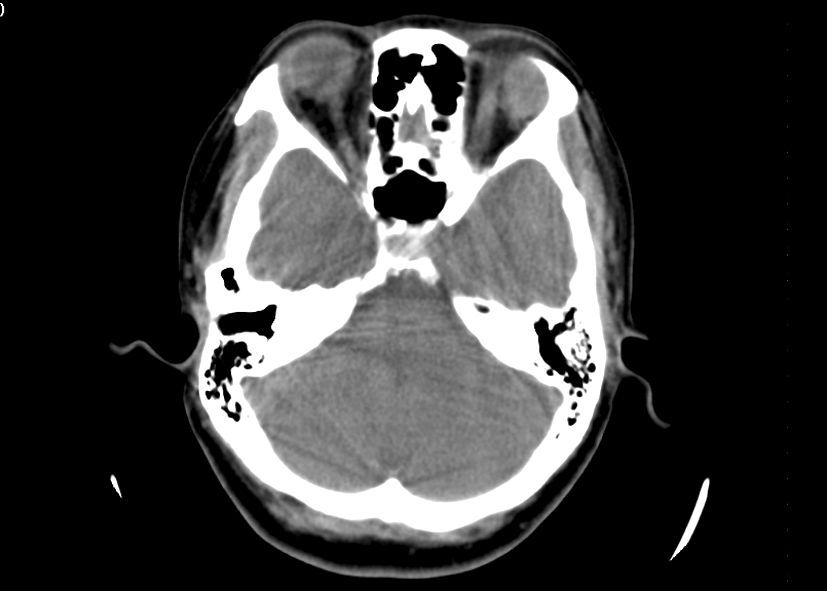
\includegraphics[width=.7\textwidth,height=\textheight,keepaspectratio]{./images/Image00104.jpg}
 \captionsetup{justification=centering}
 \caption{左侧泪腺区良性肿瘤}
 \label{fig3-6}
  \end{figure} 

\textbf{【鉴别诊断】}
炎性肿块边缘欠清,无骨质破坏,可伴筛窦黏膜增厚和眶内侧软组织增厚,应注意鉴别。

\subsection{眶内神经鞘瘤}

本病主要起源于眶内感觉神经(眼神经及其分支)鞘膜,是由雪旺氏细胞形成的良性肿瘤,极少数恶变,占眶内肿瘤的1%~6.4%,大约1.5%~1.8%伴神经纤维瘤病。

\textbf{【病理】}
一般为单发球形或椭圆形肿块,外有完整包膜,肿瘤内有囊变和出血,极少数恶变。神经鞘瘤主要由梭形细胞组成,并有疏松黏液样区和高脂质。即与其他神经鞘瘤一样,瘤内同时包括Antoni
A型细胞构成的实性细胞区及Antoni B型细胞构成的疏松黏液样组织区。

\textbf{【临床表现】}
以中年多见。缓慢进行性无痛性眼球突出为常见表现,可有视力损害和复视、斜视,可压迫视神经致视乳头水肿、视野缺损和视神经萎缩。

\textbf{【CT表现】}
表现为球后肿块,可位于肌锥内、外间隙,但以上直肌上方的肌锥外间隙为多(与感觉神经分布有关)。平扫呈等密度圆形或椭圆形肿块,与颅内沟通时呈哑铃状,边缘光滑,与眼外肌呈等密度,常有囊变、出血,罕有钙化。增强扫描可呈明显均匀强化,较大肿瘤出现囊变,而呈环状均匀或不均匀强化,这也是与血管瘤的主要鉴别点。肿瘤压迫可使眶骨发生变形或骨质缺损。少数包绕视神经生长而难与视神经鞘脑膜瘤鉴别。

\textbf{【鉴别诊断】}
眼眶内神经鞘瘤应注意与视神经胶质瘤、眶内脑膜瘤及眶内血管瘤(见表\ref{tab3-4})相鉴别。

\begin{table}[htbp]
\centering
\caption{眶内神经鞘瘤与视神经胶质瘤、眶内脑膜瘤及眶内血管瘤的鉴别}
\label{tab3-4}
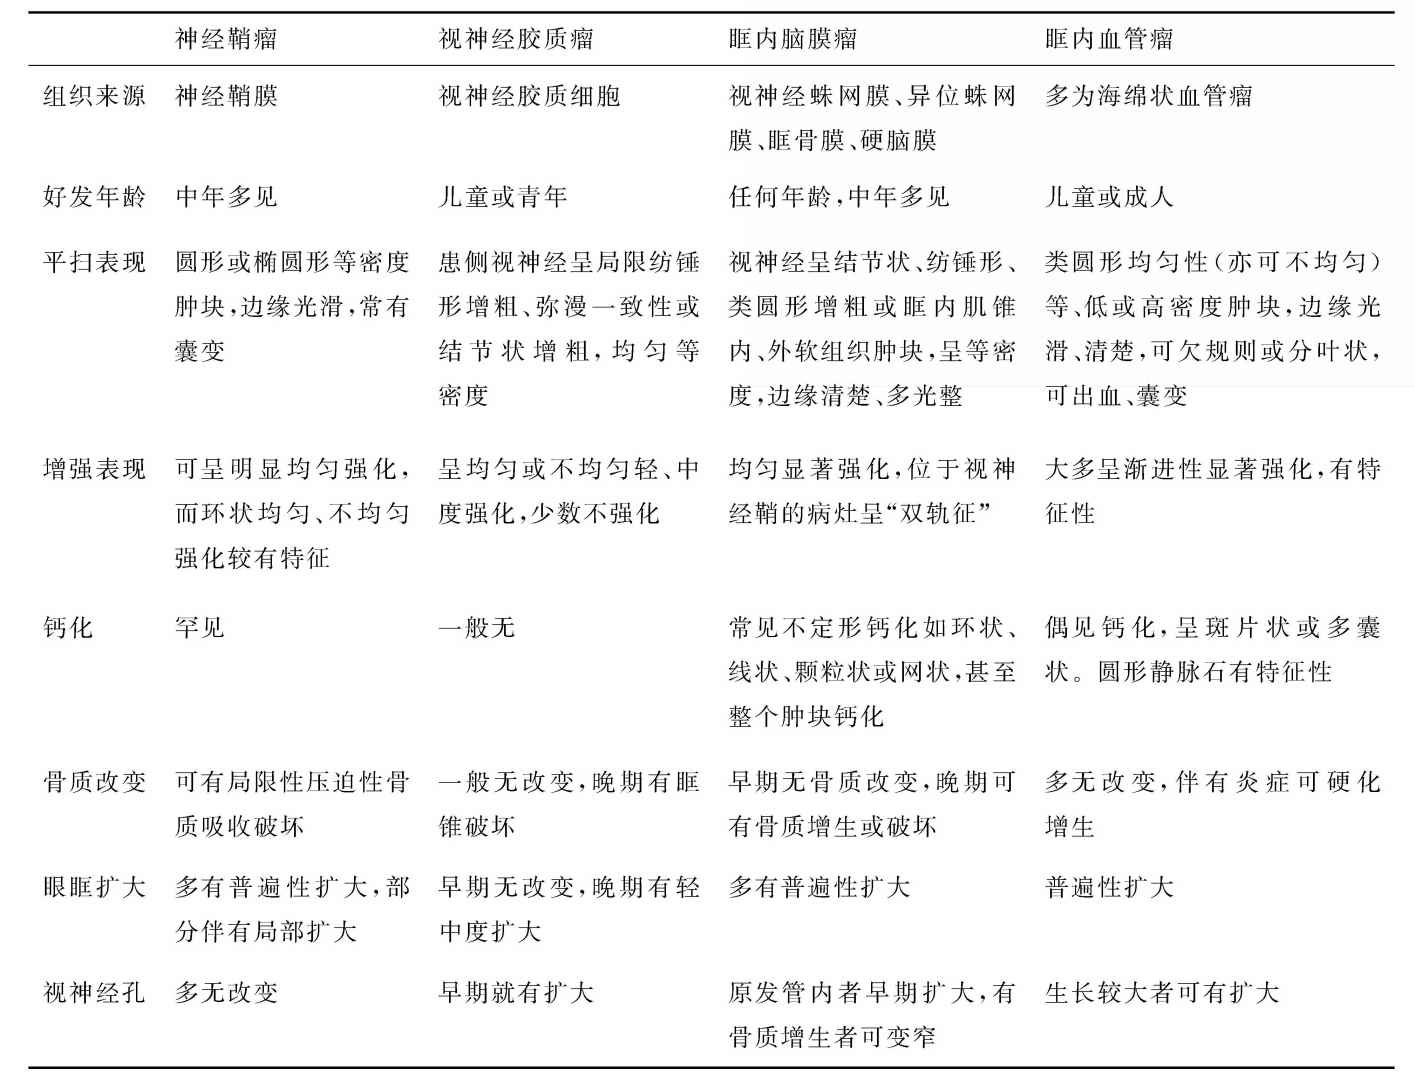
\includegraphics[width=\textwidth,height=\textheight,keepaspectratio]{./images/Image00105.jpg}
\end{table}

\subsection{眶内神经纤维瘤}

本病由周围神经的多种成分过度增生构成,通常以纤维组织和鞘膜细胞增生为主,伴有血管增生。

\textbf{【病理】}
可分为3型:①丛状神经纤维瘤:是神经纤维瘤病的特殊病症。②弥漫性神经纤维瘤:较少伴有神经纤维瘤病,是外周神经鞘成分的浸润性增生,可代替眶脂肪,侵入眼外肌,很多病变为实性,有的黏液变性为主。③局限性神经纤维瘤:为局限生长的病变,可有假包膜,而无真正的神经束膜。

\textbf{【临床表现】}
丛状神经纤维瘤和弥漫性神经纤维瘤多见于10岁以前;局限性神经纤维瘤多见于20~50岁。临床主要表现为眼球突出、斜视和视力下降等症状。

\textbf{【CT表现】}
丛状神经纤维瘤呈丛状软组织样密度灶;弥漫性神经纤维瘤呈界限不清的软组织肿块;局限性纤维瘤呈边界清楚的椭圆形肿块或呈长扁形肿块。肿块与眼外肌等密度,密度均匀或不均。增强后肿块轻到中度不均匀强化。少数神经纤维瘤可发生恶变,而出现广泛浸润眶内结构等表现。

\textbf{【鉴别诊断】}
①弥漫性神经纤维瘤需与炎性假瘤或淋巴瘤鉴别。弥漫性神经纤维瘤病史较长,且多在10岁以前就开始发病有助于鉴别。②局限性神经纤维瘤需与神经鞘瘤鉴别。后者多有囊变有助于鉴别,但有时鉴别困难。

\subsection{眼眶表皮样囊肿和皮样囊肿}

本病发生于眼眶的囊肿大多属发育性囊肿,包括皮样囊肿、表皮样囊肿和畸胎瘤,其他偶见的有泪腺潴留囊肿、血囊肿、植入性囊肿、寄生虫囊肿和先天性小眼球伴囊肿等。此外,鼻窦黏液囊肿、骨囊肿、脑膜脑膨出等亦可扩展至眼眶内。表皮样囊肿和皮样囊肿两者占眶内肿物的2.2%~9.2%。

\textbf{【病因病理】}
表皮样囊肿和皮样囊肿两者是胚胎期异位上皮组织形成的囊肿,部分表皮样囊肿由外伤后表皮样组织植入眶内所致。囊肿壁由角化的复层鳞状上皮构成,囊内有片状角化蛋白。如囊壁外层有皮脂腺和毛根称为皮样囊肿;如囊肿无皮肤附件结构则称为表皮样囊肿。畸胎瘤含有3种胚胎组织,很少见。

\textbf{【临床表现】}
常在儿童期就引起眼球突出。在眶缘可触及肿块,如无感染或出血,一般生长缓慢。

\textbf{【CT表现】}
多位于肌锥外,少数位于肌锥内。一般先天性表皮样囊肿位于眼睑或眶周皮肤内;皮样囊肿多起源于眼眶外上方之颅缝内或眶周,少数沿鼻额缝生长而位于眼眶内上方,甚至泪囊区。典型表现为圆形、椭圆形或哑铃状低密度肿块,皮样囊肿密度不均,常有负CT值区,提示含有脂肪。囊壁与眼外肌等密度,部分囊肿壁有钙化。少数皮样囊肿内密度与眼外肌密度相等。囊肿常位于眶骨缝并可引起眶骨骨质缺损,周围骨质常有硬化边缘。增强扫描囊肿壁轻至中度环状强化。

\subsection{眶内转移瘤}

儿童发生眼眶转移瘤的机会多于眼球,常见的原发肿瘤是神经母细胞瘤和尤文氏瘤,还有白血病。成人转移瘤多累及眼球(见前),原发癌以乳癌、肺癌较常见,其次为胃癌、前列腺癌等。此外,鼻窦和鼻咽部恶性肿瘤也可直接侵犯眼眶。

\textbf{【临床表现】}
主要为眼球突出、眼眶痛、眼球运动障碍、视力减退等,儿童患者症状发生迅速,可有原发肿瘤的相应症状。

\textbf{【CT表现】}
眶内转移瘤60%位于肌锥外,20%位于肌锥内,20%为弥漫性;约2/3伴有眶骨改变。转移瘤可为多灶性局限性肿块,亦可呈单发的圆形或椭圆形肿块,以及眶内弥漫性肿块。肿块密度可均匀,也可不均匀,与眼外肌等密度,边缘较模糊。增强后轻至中度强化。眶壁骨质破坏大多为溶骨性,少数为成骨性(如前列腺癌),甚至混合性。

本病需与炎性假瘤、淋巴瘤、格氏病、横纹肌肉瘤及其他眶内肿瘤鉴别。

\subsection{眶内肉瘤}

眶内中胚叶组织起源的肉瘤并不多见,但其病理类型较多如横纹肌肉瘤、淋巴肉瘤、未分化肉瘤、纤维肉瘤、脂肪肉瘤、软骨肉瘤、成骨肉瘤、滑膜肉瘤等。其中,以横纹肌肉瘤和淋巴肉瘤较为常见。横纹肌肉瘤是儿童眼眶原发恶性肿瘤中较常见的一种,淋巴肉瘤则多发生在中年,其他肉瘤常为儿童和青年多见。

\textbf{【临床表现】}
①横纹肌肉瘤80%以上发生在10岁以下儿童,男性略多。一般多为单侧发病,发病特点为起病急、发展快。主要表现为高度眼球突出、眼睑及球结膜水肿、眶部疼痛、眶缘部扪及肿块等。②淋巴肉瘤发病较为缓慢,常为继发性。可发生于双眼,表现为对称性、无痛性、进行性突眼及眼睑水肿等。

\textbf{【CT表现】}
眼眶肉瘤可发生于眼眶内任何部位,多呈浸润性生长。多表现为不规则、边缘尚清的软组织肿块。平扫显示为均匀等密度或等、低混合密度;增强扫描呈均匀或不均匀强化。肿瘤常侵及肌锥内结构,亦可侵及骨质出现局部骨质破坏。

眶内横纹肌肉瘤和淋巴肉瘤两者在CT上较难鉴别,多依赖活检。

\subsection{眼眶绿色瘤}

本病是儿童中较为常见的眼眶肿瘤,是急性髓性白血病异常细胞在眼眶骨膜下或软组织内形成的局限性浸润,因肿瘤呈淡绿色而得名。少数亦可见于慢性粒细胞白血病和单核细胞白血病。

\textbf{【临床表现】}
本病多见于10岁以下的儿童,亦可见于青年或其他年龄,男性居多。病变常在血象异常前数月出现,常双眼同时或先后受累,起病急、发展快。主要表现为眼睑、结膜肿胀,眼球运动障碍和突眼,于眶缘可见绿色肿块,常伴出血和疼痛等。

\textbf{【CT表现】}
边缘清楚的结节状肿块,平扫呈等密度或略高密度,增强扫描呈中度均匀强化。肿瘤常侵犯眶壁骨膜、骨质,骨膜形成新月状外观或伴破坏,且可见骨质溶骨性破坏,常有眼球突出。应注意与神经母细胞瘤眶内转移相鉴别。

\subsection{眼睑恶性肿瘤}

眼睑良性肿瘤种类很多且一般不侵犯眶骨,故影像学检查多无重要意义。眼睑恶性肿瘤可侵及眼球和眼眶。

\textbf{【临床表现】}
①眼睑基底细胞癌发病率最高,约占50%以上,好发于下睑内眦部。多见于老年人,男性略多。②睑板腺癌发病率约占30%,上睑约为下睑的3倍,病人多为老年女性。③鳞癌及恶性黑色素瘤较少。眼睑恶性肿瘤常呈菜花状肿块,表面糜烂,常继发感染,可侵及眼球甚至破坏眶骨、淋巴转移。

\textbf{【CT表现】}
各类眼睑恶性肿瘤均可表现为眼睑局部增厚或结节状软组织肿块,较大肿瘤可向前突起,或向后侵及眼球、眶内软组织和眶骨。肿瘤边缘尚清但不规则,密度均匀,增强扫描呈均匀或不均匀强化。有时可见眶骨破坏。

\section{眶内血管性病变}

\subsection{眶内血管瘤}

本病是眶内较常见的良性肿瘤,并常认为海绵状血管瘤是最常见的眶内肿瘤。病理分为两大类:①多形性组成:实际是一类胚胎期脉管组织发育畸形,包括毛细血管瘤、海绵状血管瘤、静脉性血管瘤、蔓状血管瘤和淋巴血管瘤;②单形性真性肿瘤:包括血管内皮瘤、血管外皮瘤和血管平滑肌瘤,但以毛细血管瘤和海绵状血管瘤好发于眶内及眼睑,其次为静脉性血管瘤较常见。

\textbf{【病理】}
①毛细血管瘤相对较少见,由毛细血管和内皮细胞增殖而成,一般无包膜。大多位于眼睑,少数可在眶内生长。②海绵状血管瘤较多见,由大小不等的血管腔构成,内有红细胞,有完整包膜。早期多原发于肌锥内,以后可穿出至肌锥外生长。肿块与周围组织常有粘连,可有出血、囊变及血栓形成,晚期可有纤维化及钙化。

\textbf{【临床表现】}
毛细血管瘤多发生于1岁以内的婴儿;海绵状血管瘤可见于任何年龄,以20~40岁青壮年多见。眶内血管瘤主要表现为眼球突出及偏位,在低头或哭泣时可有突眼加重。可经眶缘触及具有压缩性的肿块,偶有搏动及杂音。视力损害多较缓慢。肿块可因破裂出血或继发炎症而短期内增大。

\textbf{【CT表现】} 两者表现如下:

1.毛细血管瘤:病变多位于肌锥外、眶隔前、眼睑深部,较大肿瘤可延伸至视神经管、眶上裂及颅内。平扫呈边缘欠清的肿块,密度均匀或不均,较少见到钙化。增强后呈轻至中度不均匀强化。

2.海绵状血管瘤:肿瘤大多位于肌锥内,其次为肌锥外,有少数位于眶骨内或眼外肌内,一般不累及眼球和视神经。平扫呈边缘清楚的圆形、类圆形或分叶状肿块。肿块密度依其血窦和间质的多少可为高、低、等不同密度,密度均匀或不均。部分病例可见斑点状钙化,如为圆形钙化则提示为静脉石形成。增强扫描(于25~30秒行动脉期、60~70秒行静脉期、4~5分钟行延迟扫描)呈缓慢进行性显著强化为其特征性表现。多见早期呈局部小片状强化,延迟扫描逐渐强化充填,10~20分钟后呈完全均匀强化,5~10分钟维持在最高水平(CT值可达100Hu以上),20分钟后CT值开始下降。其缓慢进行性显著强化的特点有助于与其他血供丰富的肿瘤相鉴别(图\ref{fig3-7})。

\begin{figure}[!htbp]
 \centering
 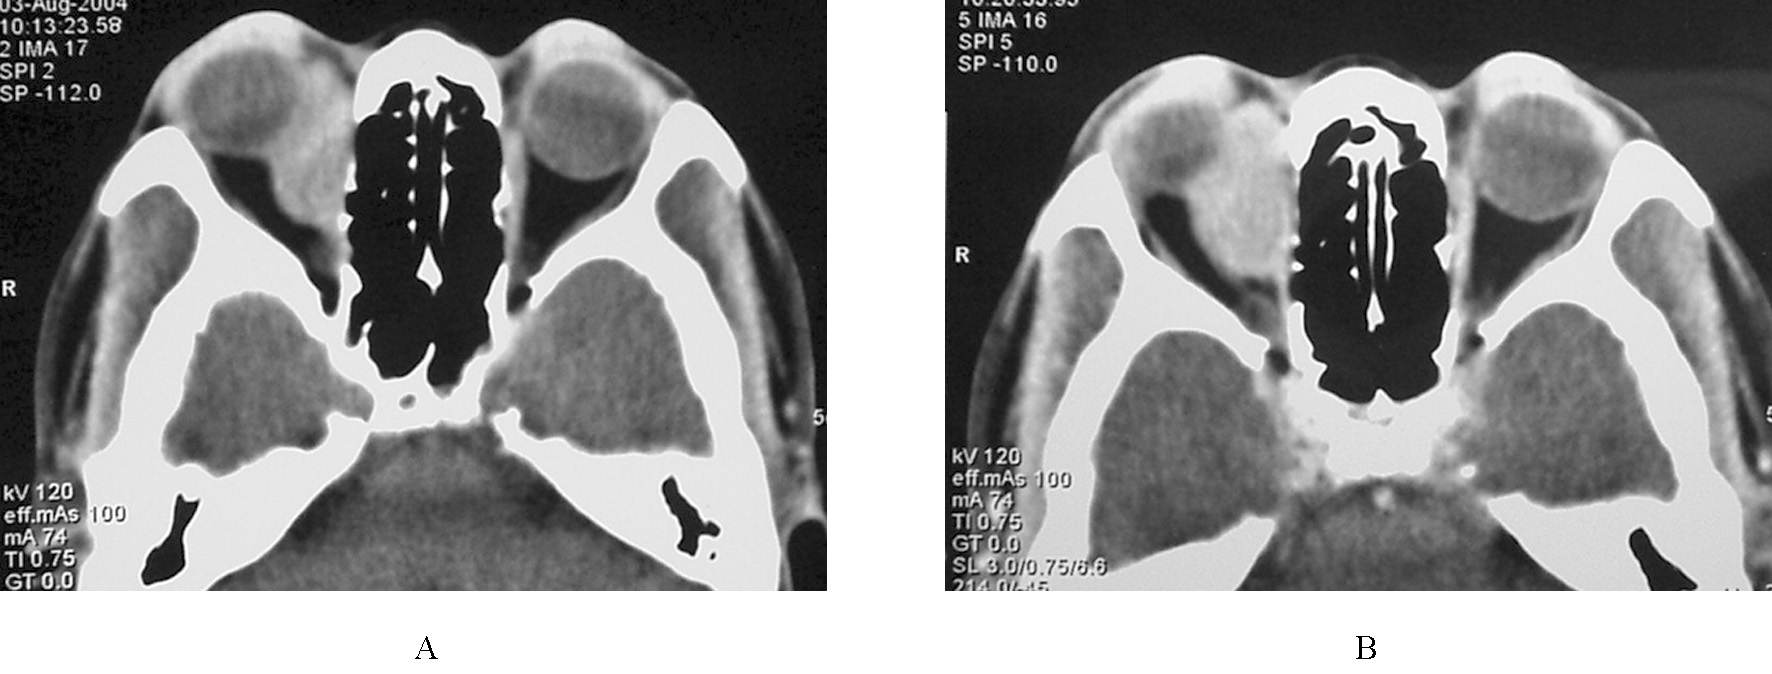
\includegraphics[width=.7\textwidth,height=\textheight,keepaspectratio]{./images/Image00106.jpg}
 \captionsetup{justification=centering}
 \caption{眶内血管瘤\\{\small A、B为同一患者,A为平扫,B为增强扫描,右侧眶内软组织肿块,显著强化}}
 \label{fig3-7}
  \end{figure} 

\textbf{【鉴别诊断】}
海绵状血管瘤主要应与静脉性血管瘤相鉴别。后者本质为静脉扩张畸形,与体静脉相通。部分病例随体位、Valsalva's试验、压迫颈部使静脉压升高而增大。两者均有明显强化,但有以下区别:①静脉性血管瘤中可见粗大的血管影或延迟扫描不能完全填充;而海绵状血管瘤多完全填充。②两者CT值达高峰的时间有差异,即多数静脉性血管瘤增强后即刻达高峰;而多数海绵状血管瘤在增强后5分钟才达高峰。③两者增强后30分钟延迟扫描,静脉性血管瘤的CT值下降较海绵状血管瘤明显,说明了静脉性血管瘤较海绵状血管瘤血管丰富、直接,引流也较好。

\subsection{眶内淋巴管瘤}

本病多发生于儿童期,肿瘤在生长期逐渐长大。

\textbf{【病理】}
为无包膜不规则肿块,其组织学为无包膜、弥漫浸润性病变,由大小不等的淋巴管组成,腔内为清亮的淋巴液。

\textbf{【临床表现】}
主要为眼球突出,而且波动性大,若瘤内有自发出血可产生巧克力囊肿,而致眼球明显突出。

\textbf{【CT表现】} 可分为弥漫性和局限性两种。

1.弥漫性:呈广泛累及眼睑软组织、肌锥内外结构的弥漫性肿块,界限不清楚,密度不均匀,囊腔内如有新鲜或陈旧出血则为略高密度或囊性低密度区,少数瘤内有钙化。增强后一般不强化或仅有小部分区域强化。

毛细血管瘤一般累及眶隔前且增强后明显强化,有助于鉴别。但如累及眶隔后,且淋巴管瘤也可有强化则难以鉴别。

2.局限性:呈圆形或椭圆形肿块,密度与眼外肌等密度,可均匀或不均匀。增强呈轻度至明显均匀或不均匀强化。有时与海绵状血管瘤很难鉴别。

\subsection{眶内静脉曲张}

本病有原发和继发两类。多为先天性静脉血管异常,是由于血管壁的先天性薄弱而导致;少数为继发性,多继发于颅内或眶内动静脉瘘。

\textbf{【临床表现】}
大多见于青年,常为单侧,尤以左侧多见,亦可为双侧。特征性表现为间歇性突眼,在低头、屏气、咳嗽、压迫静脉或做Valsalva's试验时,由于静脉回流障碍而迅速眼球突出,眶周静脉常见增粗,卧位时消失或减轻。病程长者因眶内脂肪萎缩亦可出现眼球凹陷,伴有动静脉瘘者有搏动性突眼。

\textbf{【CT表现】}
平扫显示为边缘较清楚的条状、网状或不规则团块状软组织密度影;少数可见到眶内小圆形高密度静脉石。增强后曲张静脉明显强化,如其内有血栓形成则局部无强化。眼球突出可因体位或压力变化有较快变动;眼外肌可有受压表现;伴发颈内动脉海绵窦瘘时,可见受累海绵窦扩大(图\ref{fig3-8})。

\begin{figure}[!htbp]
 \centering
 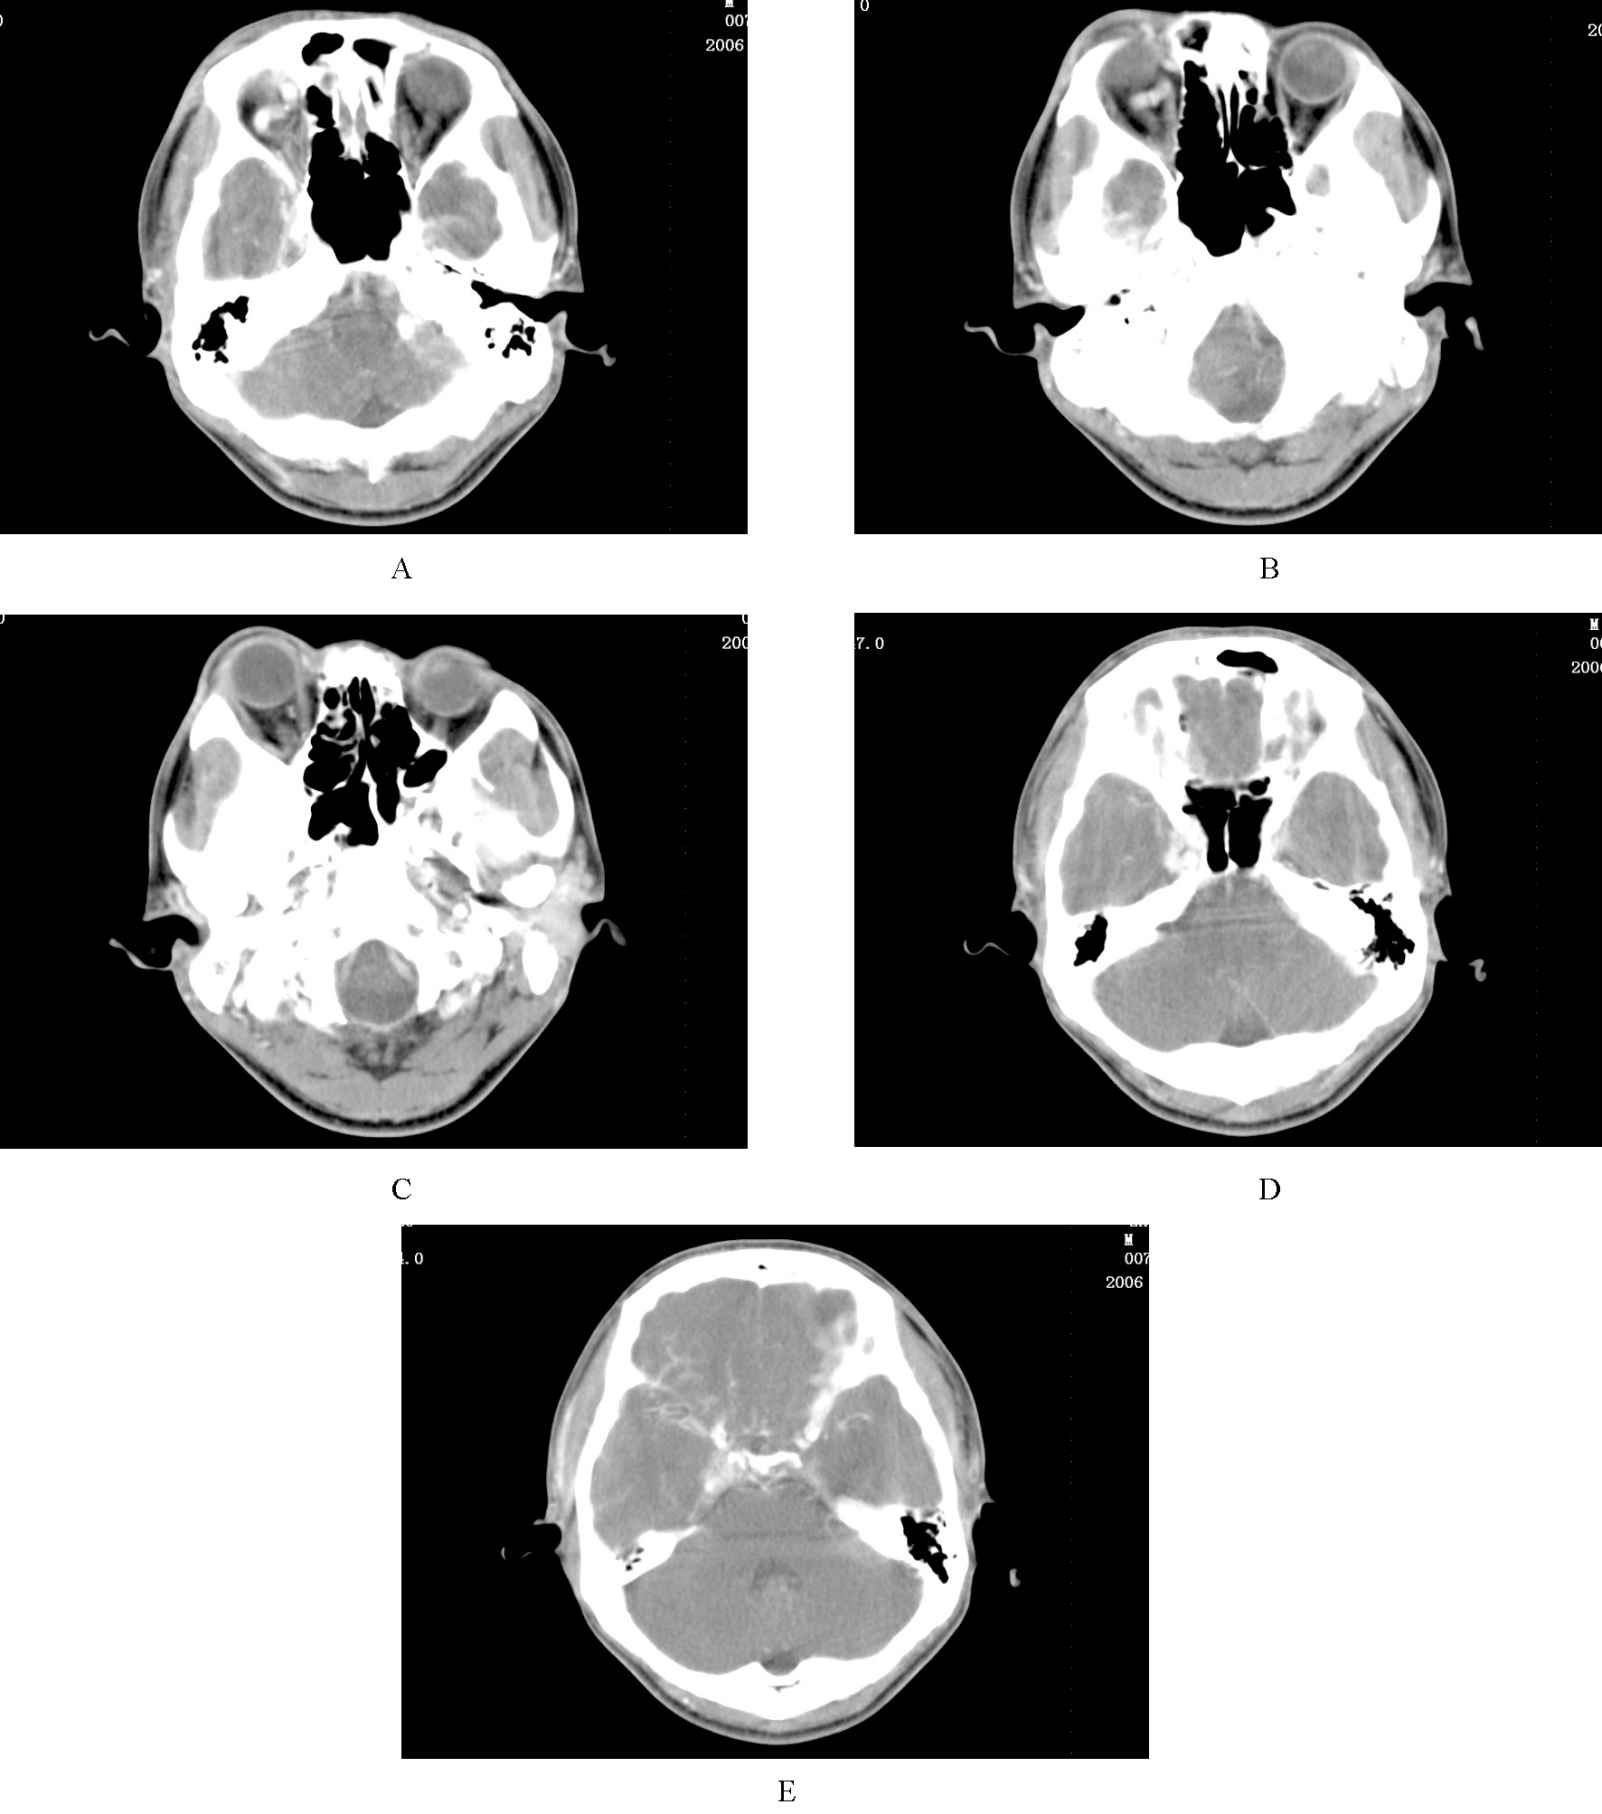
\includegraphics[width=.7\textwidth,height=\textheight,keepaspectratio]{./images/Image00107.jpg}
 \captionsetup{justification=centering}
 \caption{颈内动脉海绵窦瘘\\{\small A~E为同一患者,A、B可见眼上静脉扩张;C可见眼外肌肥厚和眶内软组织肿胀、突眼;D、E可见右侧海绵窦扩大}}
 \label{fig3-8}
  \end{figure} 

\subsection{颈内动脉海绵窦瘘}

海绵窦为中颅凹两层硬脑膜构成的硬脑膜窦,眼上静脉、眼下静脉、蝶顶窦静脉、外侧裂静脉和基底静脉汇入其中,颈动脉穿行其间。这是体内惟一动脉通过静脉的结构。当任何原因造成颈内动脉壁破裂后,动脉血直接流入海绵窦,就形成海绵窦区动静脉瘘。根据解剖部位分为颈动脉海绵窦瘘和硬脑膜动脉海绵窦瘘,前者多为外伤性,后者多为自发性。

\textbf{【病因】}
①外伤性:多见,大多由颅底骨折所致。②自发性:病因较多,主要见于颈内动脉虹吸部动脉瘤破裂、硬膜型动静脉畸形及遗传性胶原纤维缺乏病等。此外,动脉硬化、炎症、妊娠等亦可造成自发性。

\textbf{【临床表现】}
搏动性突眼、眼睑和球结膜高度水肿、眼球运动障碍、视力下降,患者有轰轰样耳鸣,眼球上方可触及震颤或听及连续性杂音。本病病情重、难自愈,且有失明危险,需及时栓塞治疗。

\textbf{【CT表现】}
①眼球突出;②海绵窦扩大;③眼上静脉扩张。增强后更易显示扩张的海绵窦和眼上静脉(图\ref{fig3-8})。

此外,眼外肌肥厚和眶内软组织肿胀、突眼,患侧脑组织水肿、出血、脑萎缩是引流静脉压力增高及“盗血”引起的继发改变。

\textbf{【鉴别诊断】}

1.硬脑膜动脉海绵窦瘘:①颈内动脉海绵窦瘘多有外伤史,发病时间短,临床症状明显;而硬脑膜动脉海绵窦瘘多无外伤史,发病时间较长,临床症状相对较轻,可自愈。②颈内动脉海绵窦瘘的CT表现如眼球突出、眼上静脉扩张、海绵窦扩大、眼肌肥大等均较硬脑膜动脉海绵窦瘘明显,但确诊依赖于血管造影。

2.某些眼科疾病如眼眶肿瘤、炎性假瘤、血管畸形、Graves眼病、海绵窦栓塞等亦可引起眼上静脉扩张。但通常海绵窦不扩大,眼上静脉扩张不及颈内动脉海绵窦瘘明显,并且多以一种改变为主,不同时具备上述几种表现,多易鉴别。

\subsection{眼动脉瘤}

\textbf{【病因】}
本病很少见,可由眼动脉发育畸形、创伤、动脉硬化或动脉内膜炎等发展而来。多为单侧,偶可双侧发生。

\textbf{【临床表现】}
当病灶较大时,可出现眼球突出、视神经萎缩或视乳头水肿以及视野缺损,也常有复视、眼球运动障碍和眼神经麻痹等,少数还有搏动性突眼。

\textbf{【CT表现】}
眼动脉瘤的显示受着某些因素的影响,如瘤体大小、部位、瘤腔通畅情况和血栓形成情况以及动脉瘤是否破裂出血等。平扫显示动脉瘤钙化和较大动脉瘤呈现的圆形或条形略高密度影。增强多数明显均一强化,呈边缘清晰的圆形或不规则形,有时增厚的动脉瘤壁可强化。

\subsection{眶内动静脉血管畸形}

动静脉血管畸形(蜿蜒状血管瘤)是一种先天性血管异常,多数为动静脉间的异常吻合,少数可为静脉间或动脉间的异常吻合为主。可发生于眼睑、眼眶、眼和颅内,有时单独发生于眼睑和眶内,更多见于眼和颅内。

\textbf{【临床表现】}
多见于30~40岁,也可见于儿童。多为单侧发病,少数可为双侧性。眼睑病变可直接见及。眶内病变常表现为眼球突出,可有或无眼球搏动,可有眼睑及结膜水肿和血管扩张,额颞部亦可有血管增粗,眼球外方可闻及杂音并触及震颤。视网膜动静脉畸形常伴颅内同类病变,有时还可伴眶周部痣,视力和视野多有损害。

\textbf{【CT表现】}
平扫表现为局限性高、低密度或低等混杂密度区,多呈不规则的团块状或点线状,边缘不清。可有眶内环状或螺旋状钙化,偶为线状钙化,增强后病灶有强化。

\section{眼部其他疾病}

\subsection{视网膜脱离}

本病是指视网膜本身的色素上皮层与神经上皮层之间的分离。

\textbf{【病因】}
临床上可分为两类。①原发性:由于视网膜出现裂孔,变性液化的玻璃体液经裂孔进入视网膜层间,导致视网膜分离。高度近视或老年性视网膜退行性萎缩和囊变等原因是形成视网膜裂孔的病理基础。②继发性:是由于其他眼病引起的视网膜层间分离,常见于视网膜和脉络膜肿瘤、炎症、外伤等。

\textbf{【临床表现】}
患者早期多有火花、闪光感或物像颤动,之后出现视力下降、视物变形、视野缺损。眼底镜可见玻璃体混浊、视网膜灰白色隆起,血管爬行,甚至呈漏斗状全视网膜脱离。原发性可见马蹄状或圆形裂孔;继发性可发现原发肿瘤、炎症等病因。

\textbf{【CT表现】}
呈新月状、典型者呈“V”形或翼状高密度区。增强后视网膜下积液不强化,仅见脱离的视网膜强化。继发性在显示视网膜下积液的同时,可见到肿瘤、外伤等原发病因。

\textbf{【鉴别诊断】}
CT无法鉴别视网膜脱离、脉络膜脱离以及玻璃体膜与视网膜的分离,但眼底镜下有特征性改变。

\subsection{脉络膜脱离}

本病是指脉络膜和睫状体与其外面巩膜之间的分离。

\textbf{【病因】}
外伤或眼内手术等原因引起眼压突然下降,可使脉络膜血管内的液体渗出,积存于脉络膜上腔内,形成脉络膜脱离。由于眼球赤道部的后侧有进出眼球的血管和神经而起到加固作用,故脉络膜脱离常限于眼球赤道部前侧。

\textbf{【临床表现】}
本病发病初期,脱离范围仅限于睫状体和周边脉络膜,自觉症状不明显。当波及黄斑时可出现视力下降。眼底镜可见脱离的脉络膜呈棕色或褐色的半球状隆起,表面光滑,也可有多个隆起。

\textbf{【CT表现】}
可见脉络膜上腔积液,脱离的脉络膜呈新月状或半球状高密度。脉络膜脱离与视网膜脱离等难以鉴别。

\subsection{玻璃体积血}

视网膜及脉络膜血管破裂出血可向玻璃体腔引流而致玻璃体积血。

\textbf{【病因病理】}
常见为:①视网膜及脉络膜血管疾病,如糖尿病、动脉硬化、血管炎、静脉血栓等;②眼球外伤与手术;③眼球肿瘤坏死出血;④某些全身疾病,如白血病、恶性贫血等。玻璃体内的积血或炎性渗出物,若存留时间较长可形成机化膜。机化膜多游离于玻璃体内,如一端连于球壁,随眼球运动牵拉视网膜可继发视网膜脱离。大量玻璃体积血由于红细胞裂解物的刺激,可产生炎性反应而致眼球萎缩。

\textbf{【临床表现】}
与玻璃体出血的量有关,可有眼前黑影、视力减退甚至丧失。眼底镜可见红色血块。

\textbf{【CT表现】}
玻璃体出血呈略高密度区。机化膜难以显示,但如继发视网膜脱离则出现相应表现。MR对出血的观察较为敏感。

\subsection{晶状体脱位}

本病根据病因可分为先天性和后天性,根据病变程度可分为完全性和不完全性。

\textbf{【病因】}
正常晶状体借悬韧带与睫状体的睫状体突连接固定。因悬韧带先天发育不全,纤维薄弱、松弛无力,或因严重的眼外伤如眼球的顿挫伤或震荡伤等,均可引起晶状体脱离正常位置,即为晶状体脱位。

\textbf{【临床表现】}
主觉症状为单眼复视。可因影响房水的通路致青光眼;也可因摩擦或撞击睫状体,刺激房水产生过多而致眼压增高。眼球转动时可见晶状体和虹膜震颤。

\textbf{【CT表现】}
可见到眼球变形和晶状体位置异常,脱位的晶状体常位于前房、玻璃体或夹到瞳孔中央。

\protect\hypertarget{text00011.html}{}{}

